\documentclass[pdflatex,iicol,sn-apa]{sn-jnl}

\usepackage[T1]{fontenc}
\usepackage{graphicx}
\usepackage{amsmath}
\usepackage{amssymb}
\usepackage{booktabs}
\usepackage{multirow}
\usepackage{tabularx}
\usepackage{float}
\usepackage{tikz}
\usetikzlibrary{arrows.meta,calc,fit,matrix,positioning}
\usepackage{xurl}
\hypersetup{hidelinks,pdftitle={Training Parts vs. Matching Parts: A Controlled Study of Pose-Based Gait Recognition},pdfauthor={Minas Aslanyan and Levon Aslanyan},pdfkeywords={gait recognition, 2D pose, occlusion robustness, supervised contrastive learning, part-based matching, negative results},bookmarksdepth=2}
\emergencystretch=2em

\newcommand{\R}{\mathbb{R}}
\newcommand{\Lbase}{\mathcal{L}_{\mathrm{base}}}
\newcommand{\Lglobal}{\mathcal{L}_{\mathrm{gSC}}}
\newcommand{\Lpart}{\mathcal{L}_{\mathrm{pSC}}}
\newcommand{\Lptrip}{\mathcal{L}_{\mathrm{pTri}}}

\raggedbottom

\begin{document}

\title[Training Parts vs. Matching Parts for Pose Gait Recognition]{Training Parts vs. Matching Parts: A Controlled Study of Pose-Based Gait Recognition}

\author*[1]{\fnm{Minas} \sur{Aslanyan}}\email{minas.aslanyan@iiap.sci.am}
\author[1]{\fnm{Levon} \sur{Aslanyan}}\email{lasl@sci.am}

\affil[1]{\orgname{Institute for Informatics and Automation Problems, National Academy of Sciences of the Republic of Armenia (IIAP)}, \orgaddress{\city{Yerevan}, \country{Armenia}}}

\abstract{Local anatomical features can contribute to gait retrieval without receiving
a separate identity objective. We examine this distinction on two-dimensional
pose sequences from the Chinese Academy of Sciences' Institute of Automation
gait dataset B (CASIA-B). A controlled study trains one multistream graph
backbone under six objectives and three seeds on identity-disjoint development
data. Adding part supervised contrastive learning reduces mean Rank-1 under
synthetic joint missingness from 63.90\% to 57.78\%; the paired difference is
$-6.12$ percentage points with a crossed 95\% bootstrap interval of
$[-10.29,-2.00]$. In frozen baseline checkpoints, replacing untrained local projections
with normalized raw part pools raises this endpoint to 68.23\%, a gain of
$+4.32$ points, $[+2.89,+5.71]$. Ten random-head controls and a uniform-weight
ablation distinguish this matching benefit from projection initialization and
confidence gating. With a fixed recipe, five full-training runs increase
standard-protocol Rank-1 from $48.35\pm1.85$\% to $54.04\pm2.18$\% on the
official 50-identity test split. This split was examined in earlier project
experiments, so the result demonstrates within-dataset transfer rather than
independent confirmation. Uniform and reliability-weighted raw matching attain
the same average. The results support evaluating local matching separately from
local supervision; their extension to stronger backbones, other datasets, and
real occlusion remains untested.}

\keywords{gait recognition, 2D pose, occlusion robustness, supervised contrastive learning, part-based matching, negative results}

\maketitle

\section{Introduction}

Pose-based gait recognition retrieves identities from joint trajectories,
offering a compact representation with reduced dependence on clothing,
background, and illumination \citep{liao2020posegait}. Graph encoders such as
ST-GCN, GaitGraph, and GaitGraph2 make the spatial and temporal structure of this
input explicit \citep{yan2018stgcn,teepe2021gaitgraph,teepe2022gaitgraph2}.
However, recognition depends on the evidence recovered by the pose estimator.
Occlusion and detector failures can remove joints or produce incorrect tracks;
partial body evidence is consequently a central challenge
\citep{li2024survey,huang2024occluded}.

Anatomical features offer two distinct interventions. During training, a local
identity objective can encourage each body region to discriminate individuals.
During retrieval, local similarities can supplement a global sequence score.
These interventions are often bundled, although a region that provides useful
complementary matching evidence need not be independently discriminative under
a local loss. Supervised contrastive learning supplies a plausible local
objective \citep{khosla2020supervised}, but its benefit for gait parts is an
empirical question. Separating training from matching is therefore necessary
for attributing any improvement to the intended intervention.

We examine this distinction using one fixed multistream graph backbone and
synthetic missing-joint protocols. A $2\times2$ comparison of global and part
supervised contrastive terms is supplemented by part-triplet and ungated-loss
controls, giving six objectives trained with three seeds. Input representation,
augmentation, batch construction, base identity losses, validation selection,
and evaluation masks are shared. A second study freezes the baseline
checkpoints and varies the local descriptor and scoring rule. Finally, five
runs with a fixed full-training recipe evaluate the selected descriptor on the
official CASIA-B test identities. Earlier project experiments examined those
identities; this final evaluation assesses within-dataset transfer and is not
an independently reserved test.

The study asks whether auxiliary global or part objectives improve retrieval,
whether useful local matching requires a trained projection, and whether
confidence weighting explains the matching gain. The tested part-SupCon term
reduces global-descriptor performance under synthetic corruption. Global
SupCon remains inconclusive, and the part-triplet control develops
near-collapsed local embeddings. In contrast, matching normalized raw part
pools improves clean and corrupted retrieval from the same baseline
checkpoints. Uniform and reliability-weighted matching perform similarly,
showing that the material gain is associated with local score fusion.

The contributions are:
\begin{enumerate}
    \item A controlled six-objective comparison separating auxiliary local
    supervision from retrieval scoring on a shared pose-gait backbone.
    \item Frozen-checkpoint controls that remove local projection heads,
    vary ten projection initializations and five fusion weights, and isolate
    the incremental effect of reliability weighting.
    \item Paired outcome analysis across model seeds and identities for clean,
    corrupted-probe, and corrupted-gallery endpoints, together with a five-seed
    standard-protocol evaluation of the selected matcher.
\end{enumerate}

These findings define a useful design check: evaluate a deterministic local
matcher before attributing a part-aware system's gain to auxiliary local
training. The present evidence establishes that check within this pipeline;
replication on established backbones and independent data is needed to assess
its generality.

\section{Related Work}

\subsection{Contrastive learning and local identity objectives}

SimCLR, MoCo, and supervised contrastive learning emphasize positive-pair
construction and projection geometry
\citep{chen2020simclr,he2020moco,khosla2020supervised}. Skeleton-specific
transformations and representations have supported action recognition and
person re-identification \citep{thoker2021skeleton,rao2024skeleton}.
ActCLR uses motion-dependent regions for contrastive action learning
\citep{lin2023actclr}, while GaitPT studies large-scale skeleton gait
pretraining \citep{cosma2026gaitpt}. These results motivate structured
contrastive learning; they do not determine whether an independent identity
objective is useful for each anatomical gait region.

Alignment and uniformity provide a language for embedding geometry
\citep{wang2020alignment}. BYOL and SimSiam examine alternatives to explicit
negative pairs \citep{grill2020byol,chen2021simsiam}; Barlow Twins and VICReg
address redundancy and variance \citep{zbontar2021barlow,bardes2022vicreg}.
We use variance diagnostics to identify a failure mode of the tested local
triplet objective, without inferring that these alternative objectives would
resolve it.

\subsection{Pose-gait representations and missing evidence}

PoseGait uses body pose and human priors \citep{liao2020posegait}; GaitGraph
and GaitGraph2 learn graph-based gait features
\citep{teepe2021gaitgraph,teepe2022gaitgraph2}. GPGait combines human-oriented
normalization with part-aware local--global graph extraction
\citep{fu2023gpgait}, and SkeletonGait uses skeleton maps
\citep{fan2024skeletongait}. OpenGait and FastPoseGait support standardized
and reproducible comparisons \citep{fan2022opengait,meng2023fastposegait}.
Our encoder is an internal control, not a reproduction of those systems.

Related action-recognition encoders use adaptive graphs, action-dependent
relations, multi-scale neighborhoods, shift operations, and heatmap volumes
\citep{shi2019adaptive,li2019actional,liu2020msg3d,cheng2020shift,duan2022posec3d}.
Holding an encoder fixed isolates the intervention within that encoder;
replication across these representation choices is a separate question.

Real occlusion combines missing information with incorrect localization and
misalignment \citep{li2024survey,huang2024occluded}. Occluded skeleton-action
work additionally studies imputation \citep{chen2023iopstl}. GREW and Gait3D
provide in-the-wild conditions \citep{zhu2021grew,zheng2022gait3d}, while
LidarGait examines a different geometric modality \citep{shen2023lidargait}.
Our synthetic masks isolate missingness effects and do not reproduce these
broader sources of variation.

\subsection{Part-aware representations and matching}

GaitSet pools silhouette sets, and disentangling methods separate identity
from appearance or covariates
\citep{chao2019gaitset,zhang2019disentangled,li2020disentangled}.
GaitPart, GaitGL, and 3D Local CNNs extract complementary local and global gait
features \citep{fan2020gaitpart,lin2021gaitgl,huang2021local}. Strip-based,
context-sensitive temporal, dynamic-region, and template representations offer
further spatial and temporal aggregation choices
\citep{wang2022gaitstrip,huang2021cstl,wang2023dygait,huang2025template}.
GPGait is particularly relevant because its graph structure includes local
keypoint relations \citep{fu2023gpgait}. Our narrower comparison holds the
representation architecture fixed and asks whether a local metric objective
is needed for useful local matching. It does not claim novelty for anatomical
pooling or global--local fusion themselves.

\subsection{Controlled metric-learning evaluation}

Negative sampling and pair weighting influence metric objectives
\citep{wu2017sampling,wang2019multisimilarity}. A Metric Learning Reality Check
shows why training and evaluation choices must be aligned when comparing
losses \citep{musgrave2020reality}. Multi-objective optimization and gradient
surgery motivate inspecting interactions between losses
\citep{sener2018multiobjective,yu2020gradient}. We compare objectives at fixed
settings, examine descriptor controls separately, and report gradient
agreement as a diagnostic rather than a causal explanation.

\section{Controlled Study}

Figure~\ref{fig:framework} summarizes the controlled design. Training changes
only the auxiliary objective attached to shared global or anatomical features;
the checkpoint-only control study freezes the baseline encoder and changes only
the local descriptor and matching rule.

\begin{figure*}[t]
\centering
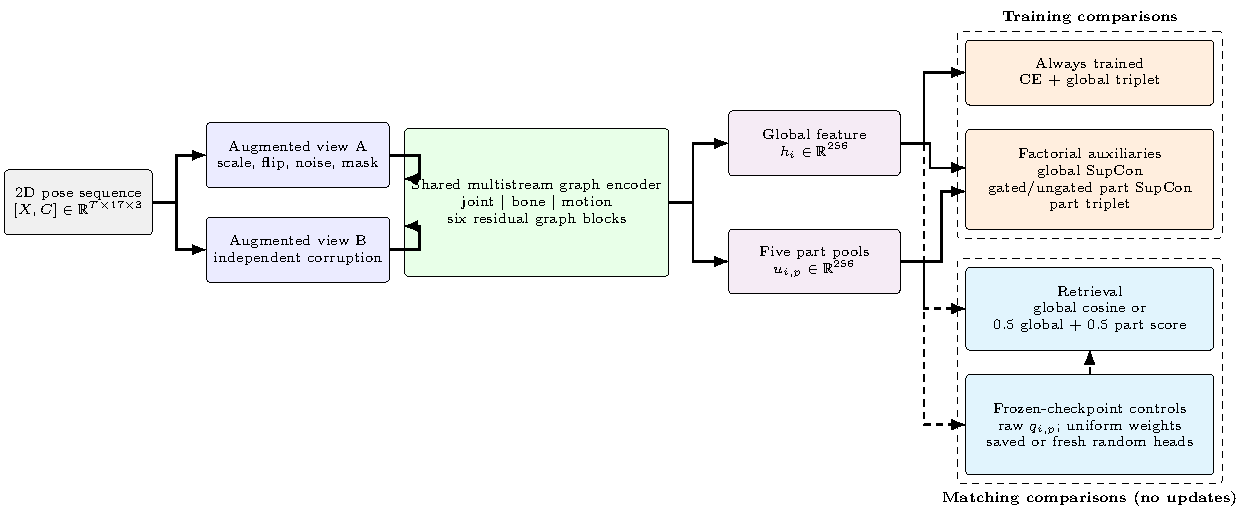
\includegraphics[width=\textwidth]{Fig1.pdf}
\caption{Separation of part-aware training from part-aware matching. Solid
arrows denote the shared forward path. The upper branch contains the six
training objectives; the lower branch contains frozen-checkpoint descriptor
controls and performs no parameter updates.}
\label{fig:framework}
\end{figure*}

\subsection{Data and identity-disjoint evaluation}

We use the public HRNet-derived \citep{sun2019hrnet} 2D pose release for CASIA-B
\citep{yu2006casia}. Each frame contains 17 joints following the COCO keypoint
convention \citep{lin2014coco}, with two coordinates and a continuous confidence
value.
For development, a fixed split seed (2026) holds out identities
\{002, 006, 012, 025, 026, 032, 043, 046, 054, 059, 061, 072\} for validation;
the remaining 62 identities train the models. For every held-out identity,
normal sequences 01--04 form the gallery and normal sequences 05--06, bag
sequences 01--02, and clothing sequences 01--02 form the probe set. This gives
792 probe sequences. Identical-view gallery entries are excluded when a probe
is scored.

The full-training evaluation uses identities disjoint from the development
validation identities. It trains
the selected metric baseline on identities 001--074 and evaluates identities
075--124. The standard single-view protocol uses normal sequences 01--04 as
gallery and normal 05--06, bag 01--02, and clothing 01--02 as probes, averages
over the 11 gallery views, and excludes identical-view matches. The resulting
test set contains 3,300 probe sequences from 50 identities. We additionally use
a pooled multi-view gallery for the controlled synthetic-corruption endpoints;
this pooled protocol is reported separately from the standard single-view score.
Earlier exploratory runs in this project evaluated the same identities 075--124.
The current development stage excludes them from checkpoint selection, but
the project history prevents describing this test population as untouched.
An external dataset is required for independent confirmation.

Coordinates are centered on the available pelvis joints, falling back to the
visible-joint centroid if the pelvis is missing, and are normalized by sequence
body scale. Confidence is supplied as a separate input and pooling weight; it
does not multiply and geometrically shrink visible coordinates. Training uses
contiguous 60-frame clips, with cyclic repetition for shorter sequences.
Evaluation uses every real frame in each sequence.

\subsection{Multistream graph backbone}

Let $X\in\R^{T\times17\times2}$ be a normalized pose and
$C\in[0,1]^{T\times17}$ its confidence. The encoder constructs three input
streams: joints $[X,C]$; bones, defined relative to a rooted skeleton parent and
observed only when both endpoints are available; and motion at lags one and two,
again retaining confidence only when both temporal endpoints are observed.
Stream-specific stems feed six residual graph blocks. Each block uses learned
perturbations of the physical adjacency and temporal convolutions with
dilations 1, 2, and 4. The hidden width grows from 64 to 256, and confidence-
weighted global pooling produces a 256-dimensional normalized embedding
$h_i$.

For local representations, we define five overlapping COCO regions: the torso
(both shoulders and hips), each arm (shoulder, elbow, wrist), and each leg
(hip, knee, ankle). Shoulder and hip joints belong to both the torso and their
respective limb; the five face joints are excluded from local pools. Confidence-weighted pooling within part
$p$ produces $u_{i,p}\in\R^{256}$. The deterministic raw descriptor is
$q_{i,p}=u_{i,p}/\lVert u_{i,p}\rVert_2$. The original learned alternative
passes $u_{i,p}$ through a part-specific two-layer projection head and
$\ell_2$ normalization to obtain $z_{i,p}$. Part reliability is
\begin{equation}
 r_{i,p}=\frac{1}{T_i|p|}\sum_{t=1}^{T_i}\sum_{j\in p}C_{i,t,j},
 \label{eq:reliability}
\end{equation}
where $T_i$ counts real rather than padded frames.

\subsection{Shared training recipe}

Each batch samples 16 identities and four sequences per identity. Two views of
each sequence receive scale, horizontal-flip, and coordinate-noise augmentation.
Each view independently has 0.3 probability of remaining geometrically complete;
otherwise one of random-joint, body-part, or temporal masking is sampled. The
maximum training severity increases linearly from 0.05 to 0.5 over the first
half of training. Dynamic-joint corruption is held out from the training
sampler and used only for evaluation.

All configurations share the base objective
\begin{equation}
 \Lbase = \mathcal{L}_{\mathrm{CE,aug}}
 +0.5\mathcal{L}_{\mathrm{CE,clean}}
 +\mathcal{L}_{\mathrm{Tri}},
 \label{eq:base}
\end{equation}
where the first term classifies both augmented views, the clean anchor classifies
the original sequence, and $\mathcal{L}_{\mathrm{Tri}}$ is batch-hard triplet
loss \citep{hermans2017triplet} on $h_i$. Same-source augmented views are excluded
as triplet positives, so positives must be distinct sequences of the same
identity.

Global supervised contrastive loss $\Lglobal$ operates on a projection of the
global embeddings and uses every same-identity view as a positive. Part
supervised contrastive loss applies the same construction independently to each
$z_{i,p}$. In the gated version, a positive pair receives weight
$r_{i,p}r_{j,p}$ and the anchor receives weight $r_{i,p}$; parts below reliability
0.05 are excluded from both positives and negatives. The ungated control gives
all parts above the same 0.05 reliability threshold unit weight. Part triplet loss $\Lptrip$ applies batch-hard
triplet independently to every present part. The complete factorial objective
is
\begin{equation}
 \mathcal{L}=\Lbase+\gamma_g\Lglobal+\gamma_p\Lpart+
 \gamma_{pt}\Lptrip.
 \label{eq:factorial}
\end{equation}

\begin{table*}[t]
\centering
\caption{Controlled training objectives. All unlisted terms and all backbone,
augmentation, and optimization settings are identical.}
\label{tab:objectives}
\small
\begin{tabular}{lrrrl}
\toprule
Configuration & $\gamma_g$ & $\gamma_p$ & $\gamma_{pt}$ & Part-SupCon gate \\
\midrule
Metric baseline & 0 & 0 & 0 & -- \\
Global SupCon & 0.2 & 0 & 0 & -- \\
Part SupCon & 0 & 0.2 & 0 & reliability \\
Part triplet & 0 & 0 & 0.2 & -- \\
Global + part SupCon & 0.2 & 0.2 & 0 & reliability \\
Global + part SupCon (ungated) & 0.2 & 0.2 & 0 & presence only \\
\bottomrule
\end{tabular}
\end{table*}

Development training lasts 160 epochs with AdamW, initial learning rate $10^{-3}$, weight
decay $10^{-4}$, five warm-up epochs, cosine decay to 1\% of the initial rate,
label smoothing 0.1, global SupCon temperature 0.07, part temperature 0.1,
triplet margin 0.2, gradient clipping at 5, and automatic mixed precision. A
checkpoint is selected every five epochs using only the held-out validation
split. The score assigns 75\% weight to clean recognition and 25\% to the mean
of body-part and random-joint recognition at severity 0.3. Selection uses only
the global descriptor for every method.

For the official-test evaluation, only the metric baseline is retrained. All 74
official training identities are used for a fixed 85 epochs with the same base
objective and optimization settings. Validation is disabled, no official test
outcome is used for checkpoint selection, and epoch 85 is evaluated for each of
five seeds (11, 22, 33, 44, and 55). The global, uniform raw-part, and
reliability-weighted raw-part descriptors are computed from each same-seed
checkpoint at the fixed 0.5 local-score weight. The 85-epoch budget is the
median selected baseline epoch in the development comparison and was fixed
before these full-training runs.

\subsection{Retrieval descriptors}

The global descriptor uses cosine similarity,
$s_g(i,j)=h_i^\top h_j$. The reliability-weighted part descriptor keeps the
same global term and averages local cosine scores over jointly reliable parts.
Let $v_{i,p}$ denote the local descriptor under evaluation: either the learned
projection $z_{i,p}$ or the normalized raw pool $q_{i,p}$. Then
\begin{equation}
 s_p(i,j)=
 \frac{\sum_p r_{i,p}r_{j,p}v_{i,p}^{\top}v_{j,p}}
 {\max(\sum_p r_{i,p}r_{j,p},10^{-8})},
\end{equation}
\begin{equation}
 s_{\mathrm{rel}}(i,j)=0.5s_g(i,j)+0.5s_p(i,j).
 \label{eq:matching}
\end{equation}
Uniform matching replaces each $r_{i,p}$ in the local score by the presence
indicator $\mathbf{1}[r_{i,p}>0]$. If no local part is jointly available,
matching falls back to $s_g$. Global and projected-part descriptors are
evaluated for every development checkpoint; raw-part controls are evaluated
for the baseline checkpoints. In particular, the metric
baseline and global-SupCon configurations give the part heads no direct loss;
their part projection weights therefore remain at their seeded initialization,
although the shared backbone changes during training.

We resolve this confound in a checkpoint-only control study. The three selected
metric-baseline backbones are frozen and each sequence is encoded once per
corruption realization. We compare (i) $q_{i,p}$ with reliability-weighted
matching; (ii) $q_{i,p}$ with uniform weights over jointly present parts; (iii)
the saved untrained heads; and (iv) ten freshly initialized frozen copies of
the same nonlinear head architecture per backbone checkpoint. No condition
updates model parameters. The local-score weight is fixed at 0.5 for the
primary comparison. We additionally report weights
$\{0,0.25,0.5,0.75,1\}$ as sensitivity analysis; they are not used to replace
the pre-specified primary weight after observing validation performance.

\subsection{Occlusion protocols and outcomes}

We evaluate random joint-frame removal, temporally smoothed dynamic-joint
removal, whole-part removal, and a contiguous temporal interruption at
nominal severities $\rho\in\{0,0.1,0.3,0.5,0.7\}$. Whole-region
masks can overlap and overshoot the requested missing-joint count, while
temporal smoothing changes the marginal dynamic-joint missingness rate.
Thus equal nominal severities do not imply equal removed-joint fractions
across families. Masks are applied to normalized poses and isolate missing
evidence rather than errors in pose estimation. Five deterministic corruption
realizations are averaged at every positive severity. In the clean-gallery
protocol only probes are corrupted. In the occluded-gallery protocol gallery
and probe sequences receive independently seeded corruption of the same family
and severity. We additionally report the CASIA-B-style single-view-gallery
average over NM, BG, and CL. Development tables use held-out training
identities; the dedicated official-test table uses identities 075--124 and is
labeled explicitly.

Figure~\ref{fig:corruptions} illustrates the four corruption families, and
Figure~\ref{fig:evaluation-matrix} records where each family appears in
training and in the two gallery protocols.

\begin{figure*}[t]
\centering
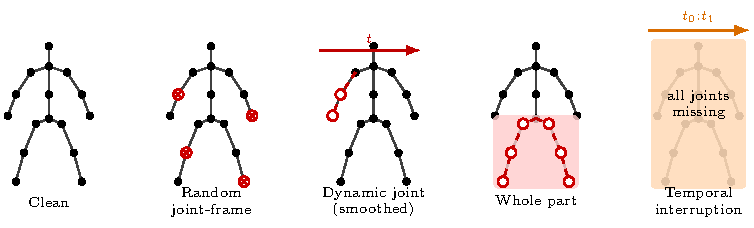
\includegraphics[width=\textwidth]{Fig2.pdf}
\caption{Conceptual corruption families. Red marks unavailable joints or body
regions; orange marks a contiguous interval in which the complete pose is
unavailable. Random joint-frame masks vary independently, whereas dynamic-joint
masks are temporally smoothed.}
\label{fig:corruptions}
\end{figure*}

\begin{figure*}[t]
\centering
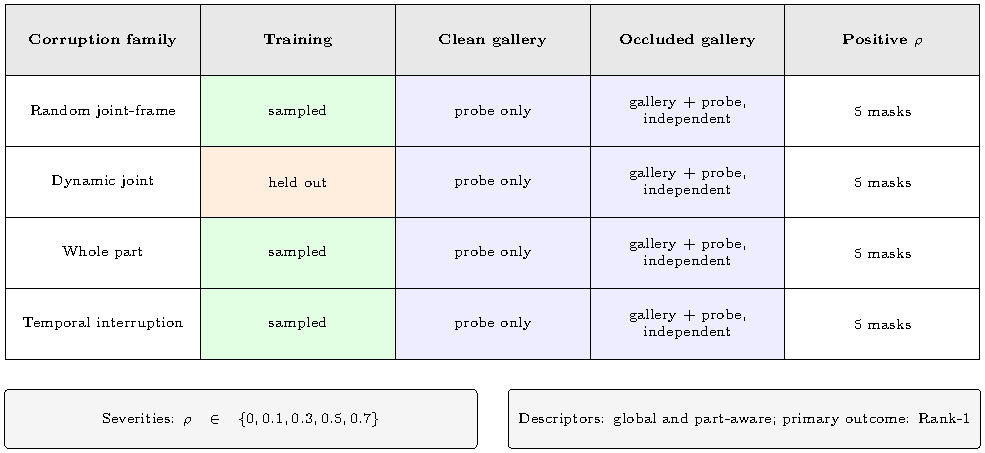
\includegraphics[width=\textwidth]{Fig3.pdf}
\caption{Evaluation matrix. Dynamic-joint corruption is deliberately held out
from training. Positive-severity results average five deterministic corruption
realizations, and gallery and probe corruptions are independently seeded in the
occluded-gallery protocol.}
\label{fig:evaluation-matrix}
\end{figure*}

The primary measure is Rank-1 retrieval. Rank-5, Rank-10, mean average
precision, equal-error rate, and true-acceptance rates are retained in the
saved run artifacts but are secondary to the present diagnosis. Development
tables report the mean and sample standard deviation over three training seeds. The main
corrupted aggregate weights the four families and four positive severities
equally; it summarizes this experimental grid, not a deployment distribution.
For paired development comparisons, each saved outcome is a per-probe correctness value,
averaged over corruption realizations where applicable. We first average the
selected corruption cells within each probe, compute candidate-minus-baseline
differences within each of 12 identities and three matched seeds, and then
resample seeds and identities as crossed factors with replacement for
100,000 draws. Each draw selects three seeds and 12 identities independently;
the same identity sample is shared across the sampled seeds because identities
recur in every model run. Candidate--baseline pairing is preserved.
Intervals are percentile 95\% intervals. They are used to express uncertainty,
not to support a confirmatory significance claim across the many exploratory
endpoints.

Official-test tables report mean and sample standard deviation over five
matched training seeds. For the standard single-view aggregate, only seed-level
paired outcomes are retained, so candidate-minus-global uncertainty is a paired
$t$ interval over the five seed differences. For pooled multi-view and
synthetic-corruption endpoints, saved per-probe outcomes support a crossed
bootstrap: five seeds and 50 test identities are independently resampled with
replacement for 100,000 draws while preserving candidate--baseline pairing.
Synthetic endpoints first average the four positive severities and four
corruption families within each probe.

\section{Results}

\begin{table*}[t]
\centering
\caption{CASIA-B validation Rank-1 (\%). Clean is mean $\pm$ seed standard
deviation. ``All $>0$'' averages four corruption families at severities 0.1,
0.3, 0.5, and 0.7. Occluded gallery averages the same positive-severity grid.
Single-view averages NM, BG, and CL. Every cell uses three training seeds.}
\label{tab:factorial-results}
\small
\setlength{\tabcolsep}{4pt}
\begin{tabularx}{\textwidth}{@{}>{\raggedright\arraybackslash}Xccccc@{}}
\toprule
\multicolumn{6}{@{}l}{\emph{Global descriptor}} \\
Training objective & Clean & \shortstack{Clean gallery\\all $>0$} &
\shortstack{Clean gallery\\$\rho=0.5$} & \shortstack{Occluded gallery\\all $>0$} &
Single-view \\
\midrule
Metric baseline & 81.52 $\pm$ 2.43 & 63.90 & 64.25 & 67.93 & 67.36 \\
Global SupCon & 79.63 $\pm$ 3.23 & 63.23 & 64.15 & 67.42 & 66.18 \\
Part SupCon & 78.79 $\pm$ 1.14 & 57.78 & 55.57 & 64.26 & 65.33 \\
Part triplet & 81.27 $\pm$ 3.41 & 60.65 & 59.10 & 66.71 & 67.82 \\
Global + part SupCon & 80.05 $\pm$ 1.34 & 60.70 & 59.06 & 65.56 & 65.75 \\
Global + part SupCon (ungated) & 80.89 $\pm$ 1.59 & 61.72 & 60.59 & 66.99 & 66.29 \\
\bottomrule
\end{tabularx}
\vspace{0.5em}

\begin{tabularx}{\textwidth}{@{}>{\raggedright\arraybackslash}Xccccc@{}}
\toprule
\multicolumn{6}{@{}l}{\emph{Projected-parts descriptor}} \\
Training objective & Clean & \shortstack{Clean gallery\\all $>0$} &
\shortstack{Clean gallery\\$\rho=0.5$} & \shortstack{Occluded gallery\\all $>0$} &
Single-view \\
\midrule
Metric baseline & 83.04 $\pm$ 1.31 & 66.31 & 67.97 & 70.57 & 69.34 \\
Global SupCon & 82.79 $\pm$ 3.36 & 66.21 & 67.85 & 70.38 & 68.66 \\
Part SupCon & 75.42 $\pm$ 2.25 & 54.66 & 52.65 & 61.62 & 61.81 \\
Part triplet & 81.31 $\pm$ 3.42 & 60.66 & 59.11 & 66.73 & 67.82 \\
Global + part SupCon & 77.86 $\pm$ 4.45 & 57.48 & 54.84 & 63.18 & 63.40 \\
Global + part SupCon (ungated) & 78.20 $\pm$ 0.07 & 59.35 & 58.11 & 64.85 & 65.60 \\
\bottomrule
\end{tabularx}
\end{table*}

\subsection{Part SupCon reduces robustness under the fixed recipe}

Table~\ref{tab:factorial-results} shows the six-objective comparison. With global
matching, the metric baseline attains 81.52\% clean Rank-1, 63.90\% averaged
positive-severity clean-gallery Rank-1, and 67.93\% when both gallery and probe
are corrupted. Global SupCon produces 79.63\%, 63.23\%, and 67.42\%,
respectively. The paired intervals in Table~\ref{tab:paired-results} include
zero for all four global-descriptor endpoints, so this experiment neither
demonstrates a benefit nor a clear robustness penalty from the global SupCon
term.

Part SupCon behaves differently. Its global descriptor loses 6.12 percentage
points on the positive-severity clean-gallery aggregate, with interval
$[-10.29,-2.00]$, and 8.68 points at severity 0.5, with interval
$[-15.55,-2.38]$. The projected-parts descriptor loses still more. Thus the
failure is not limited to a poorly chosen local matching weight: the shared
global representation also deteriorates when the local contrastive objective is
added.

\begin{table*}[t]
\centering
\caption{Paired Rank-1 difference from the metric baseline in percentage points
(crossed 95\% bootstrap interval over seed and validation identity).
Negative values favor the baseline.}
\label{tab:paired-results}
\small
\setlength{\tabcolsep}{4pt}
\begin{tabularx}{\textwidth}{@{}>{\raggedright\arraybackslash}Xlcc@{}}
\toprule
Training objective & Descriptor & Clean & \shortstack{Clean gallery,\\all $>0$} \\
\midrule
Global SupCon & Global & -1.89 [-5.30, +1.05] & -0.67 [-4.86, +3.79] \\
Part SupCon & Global & -2.74 [-6.69, +1.18] & -6.12 [-10.29, -2.00] \\
Part triplet & Global & -0.25 [-5.22, +4.17] & -3.26 [-7.59, +1.06] \\
Global + part SupCon & Global & -1.47 [-5.85, +3.03] & -3.21 [-8.97, +2.89] \\
Global + part (ungated) & Global & -0.63 [-5.35, +5.30] & -2.19 [-5.35, +1.11] \\
Global SupCon & Projected parts & -0.25 [-3.79, +2.99] & -0.10 [-3.27, +3.08] \\
Part SupCon & Projected parts & -7.62 [-11.91, -3.03] & -11.65 [-16.02, -7.32] \\
Part triplet & Projected parts & -1.73 [-6.82, +2.90] & -5.65 [-9.85, -1.16] \\
Global + part SupCon & Projected parts & -5.18 [-10.61, +0.13] & -8.83 [-14.35, -2.29] \\
Global + part (ungated) & Projected parts & -4.84 [-8.75, -1.05] & -6.96 [-11.01, -3.08] \\
\bottomrule
\end{tabularx}
\vspace{0.5em}

\begin{tabularx}{\textwidth}{@{}>{\raggedright\arraybackslash}Xlcc@{}}
\toprule
Training objective & Descriptor & \shortstack{Clean gallery,\\$\rho=0.5$} &
\shortstack{Occluded gallery,\\all $>0$} \\
\midrule
Global SupCon & Global & -0.10 [-6.13, +6.76] & -0.51 [-2.90, +1.76] \\
Part SupCon & Global & -8.68 [-15.55, -2.38] & -3.67 [-6.00, -1.27] \\
Part triplet & Global & -5.15 [-11.42, +1.28] & -1.22 [-4.29, +1.50] \\
Global + part SupCon & Global & -5.19 [-13.69, +4.17] & -2.37 [-6.16, +1.24] \\
Global + part (ungated) & Global & -3.65 [-8.91, +0.68] & -0.94 [-3.00, +1.05] \\
Global SupCon & Projected parts & -0.12 [-4.37, +4.10] & -0.20 [-2.13, +1.76] \\
Part SupCon & Projected parts & -15.32 [-22.19, -8.96] & -8.96 [-11.51, -6.03] \\
Part triplet & Projected parts & -8.86 [-15.80, -1.57] & -3.85 [-6.48, -1.32] \\
Global + part SupCon & Projected parts & -13.13 [-20.45, -4.51] & -7.39 [-11.19, -2.97] \\
Global + part (ungated) & Projected parts & -9.85 [-16.07, -4.53] & -5.73 [-8.08, -3.59] \\
\bottomrule
\end{tabularx}
\end{table*}

\subsection{Reliability gating is not the primary cause}

The combined gated objective reaches 60.70\% on the positive-severity global
aggregate. Removing reliability weights increases this to 61.72\%, and raises
the corresponding projected-parts result from 57.48\% to 59.35\%. The recovery
is directionally consistent but remains below the 63.90\% and 66.31\% metric
baselines. Average part reliability (0.502) and presence rate (0.860) are
essentially identical across methods because they are determined by the shared
input sampler. Gating therefore changes how the same observed evidence weights
the auxiliary loss; it does not explain the entire deficit.

\subsection{Part-triplet heads exhibit near-collapse}

The part-triplet control closely preserves clean global accuracy (81.27\%) but
falls to 60.65\% on the positive-severity aggregate and 59.10\% at severity 0.5.
Its projected-parts and global results are nearly identical. The training
diagnostics in Table~\ref{tab:mechanisms} are consistent with this behavior: final normalized
part variance is approximately $1.7\times10^{-6}$, and a nonzero finite
part--triplet cosine is available in only 9 of 96 scheduled diagnostics. The
other diagnostics have a zero-norm gradient for at least one compared loss;
they are not numerical failures. Training-log variance at the selected epochs (60, 60, and 40) is also
small, averaging $2.03\times10^{-6}$ across seeds and parts. These
observations support near-collapse under this particular local objective
and training recipe; they do not establish failure of part-triplet learning
in general.

Part SupCon avoids variance collapse: its final variance is
$3.34\times10^{-3}$. Nevertheless, its gradient is less aligned with the
global triplet objective than the global SupCon gradient is. In the combined
model, the mean part--triplet cosine is 0.203, compared with a global--triplet
cosine of 0.446. These cosines are positive, so the data do not support a claim
of direct gradient opposition. They instead show weaker agreement and leave
open other causes, including excessive local invariance, part-specific identity
ambiguity, or mismatch between the local contrastive task and retrieval.

\begin{table*}[t]
\centering
\caption{Training diagnostics averaged over three seeds. Part variance is the
mean coordinate-wise variance over the final 20 epochs. Cosines are measured
every five epochs; parentheses give nonzero finite cosine measurements out of
96 scheduled.}
\label{tab:mechanisms}
\small
\setlength{\tabcolsep}{4pt}
\begin{tabular}{@{}lrrr@{}}
\toprule
Objective & Variance ($\times10^{-3}$) & Part--global & Part--triplet \\
\midrule
Metric baseline & 1.269 & -- & -- \\
Global SupCon & 1.300 & -- & -- \\
Part SupCon & 3.338 & -- & 0.212 (95) \\
Part triplet & 0.002 & -- & 0.012 (9) \\
Global + part SupCon & 3.349 & 0.265 (96) & 0.203 (96) \\
Global + part SupCon (ungated) & 3.242 & 0.241 (96) & 0.195 (96) \\
\bottomrule
\end{tabular}
\end{table*}

\subsection{Raw part matching resolves the random-head confound}

\begin{table*}[t]
\centering
\caption{Checkpoint-only descriptor controls on CASIA-B validation Rank-1
(\%). All conditions use the same three selected metric-baseline backbones and
the fixed 0.5 fusion weight. ``Fresh random heads'' is the mean across ten
projection seeds; brackets give the range after averaging the three backbone
seeds. No control retrains the backbone or local head.}
\label{tab:descriptor-controls}
\small
\setlength{\tabcolsep}{3.5pt}
\resizebox{\textwidth}{!}{%
\begin{tabular}{@{}lcccc@{}}
\toprule
Descriptor & Clean & \shortstack{Clean gallery\\all $>0$} &
\shortstack{Clean gallery\\$\rho=0.5$} &
\shortstack{Occluded gallery\\all $>0$} \\
\midrule
Global only & 81.52 & 63.90 & 64.25 & 67.93 \\
Saved frozen head & 83.04 & 66.31 & 67.97 & 70.57 \\
Fresh random heads & 83.75 [83.21, 84.26] & 66.50 [66.32, 66.73] &
68.07 [67.71, 68.40] & 70.70 [70.58, 70.81] \\
Raw parts, uniform & 84.43 & 68.11 & 69.99 & 71.71 \\
Raw parts, reliability weighted & \textbf{84.47} & \textbf{68.23} &
\textbf{70.31} & \textbf{71.76} \\
\bottomrule
\end{tabular}%
}
\end{table*}

Table~\ref{tab:descriptor-controls} removes the learned projection from the
same checkpoints. Reliability-weighted raw parts improve clean Rank-1 by 2.95
points over global matching, with crossed paired interval
$[1.05,5.30]$, and improve the positive-severity aggregate by 4.32 points,
$[2.89,5.71]$. The gain grows to 6.06 points at severity 0.5,
$[3.65,8.59]$, and remains 3.83 points with independently corrupted galleries,
$[2.79,5.10]$. Every training seed improves on both clean and corrupted-probe
endpoints, and the four family-specific corrupted aggregates all increase.

All ten fresh random-head seeds also pass the clean and robustness thresholds:
their clean gains range from 1.68 to 2.74 points and their corrupted-probe gains
from 2.42 to 2.82 points. Thus the original improvement did not depend on one
favorable initialization. However, removing the nonlinear projection is both
deterministic and stronger. The effect is also insensitive to moderate fusion:
raw reliable parts improve the corrupted aggregate by 2.30, 4.32, and 5.68
points at weights 0.25, 0.5, and 0.75, respectively. We retain 0.5 as the
declared primary weight rather than selecting 0.75 after observing validation.

Reliability weighting is not the main source of the raw-descriptor gain.
Relative to uniform averaging, it changes clean Rank-1 by only $+0.04$ points
and the principal corrupted aggregate by $+0.12$ points. The crossed interval for the latter difference,
$[-0.02,+0.24]$, includes zero. The small mean difference arises mainly under
whole-part corruption. These comparisons associate the material gain with
regional pooling and score fusion; random-region controls would be needed to
attribute it specifically to anatomical grouping.

\begin{figure*}[t]
\centering
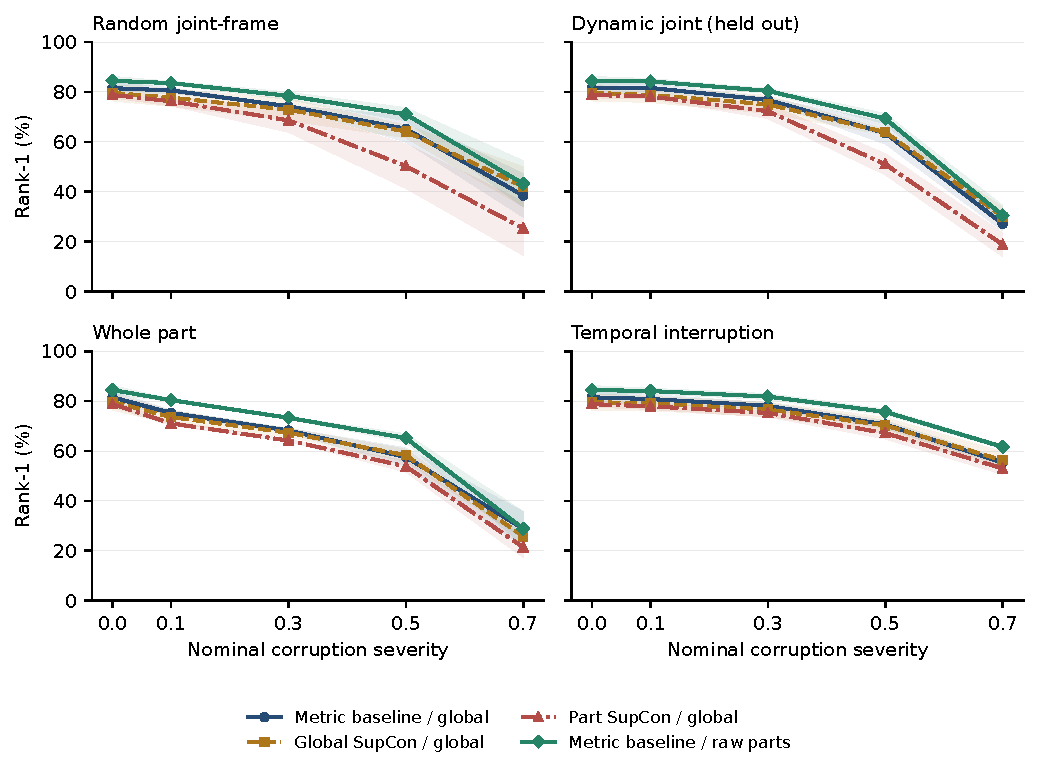
\includegraphics[width=\textwidth]{Fig4.pdf}
\caption{CASIA-B development severity curves with a clean pooled multi-view
 gallery. Lines are means over three training seeds; shaded bands show one
 sample standard deviation across seeds, not confidence intervals. Positive
 severities average five deterministic mask realizations. The raw-part matcher
 uses the same metric-baseline checkpoints at fusion weight 0.5. Severity is
 nominal and is not calibrated to equal missing-joint fractions across families.}
\label{fig:severity-curves}
\end{figure*}

Figure~\ref{fig:severity-curves} disaggregates the corruption endpoint by
family and severity. The curves show where global matching, the auxiliary
objectives, and raw-part fusion differ, including the dynamic family omitted
from training. An aggregate improvement should therefore be interpreted
alongside these family-specific accuracy profiles.

\subsection{Official CASIA-B test evaluation}

\begin{table*}[t]
\centering
\caption{Five-seed CASIA-B official-test Rank-1 (\%), reported as mean
$\pm$ sample standard deviation. The upper panel follows the standard
single-view-gallery protocol and excludes identical views. The lower panel uses
the separately labeled pooled multi-view gallery; ``synthetic'' averages four
corruption families at severities 0.1, 0.3, 0.5, and 0.7.}
\label{tab:official-test}
\small
\setlength{\tabcolsep}{3.5pt}
\begin{tabular}{@{}lcccc@{}}
\toprule
\multicolumn{5}{@{}l}{\emph{Standard single-view protocol}} \\
Descriptor & NM & BG & CL & Average \\
\midrule
Global only & $67.64\pm2.83$ & $49.50\pm1.92$ & $27.91\pm0.94$ & $48.35\pm1.85$ \\
Raw parts, uniform & $74.02\pm3.04$ & $55.56\pm2.04$ & $32.54\pm1.88$ & $54.04\pm2.21$ \\
Raw parts, reliability weighted & $74.14\pm3.04$ & $55.47\pm2.01$ & $32.52\pm1.81$ & $54.04\pm2.18$ \\
\bottomrule
\end{tabular}
\vspace{0.5em}

\begin{tabular}{@{}lccc@{}}
\toprule
\multicolumn{4}{@{}l}{\emph{Pooled multi-view controlled endpoints}} \\
Descriptor & Uncorrupted & \shortstack{Synthetic,\\clean gallery} &
\shortstack{Synthetic,\\occluded gallery} \\
\midrule
Global only & $68.06\pm0.50$ & $48.90\pm0.63$ & $54.34\pm0.63$ \\
Raw parts, uniform & $74.76\pm0.47$ & $55.13\pm1.22$ & $59.88\pm0.90$ \\
Raw parts, reliability weighted & $74.64\pm0.45$ & $55.29\pm1.22$ & $59.96\pm0.90$ \\
\bottomrule
\end{tabular}
\end{table*}

Table~\ref{tab:official-test} evaluates the selected matcher without changing
the selected objective, descriptor, or fusion weight. On the standard protocol,
reliability-weighted raw parts improve the three-condition average over global
matching by 5.69 percentage points; the paired five-seed 95\% interval is
$[5.19,6.20]$. The condition-specific gains are 6.50 points for NM,
$[6.16,6.84]$; 5.97 for BG, $[5.73,6.22]$; and 4.61 for CL,
$[3.51,5.71]$.

The saved test-identity outcomes additionally permit identity resampling for
the pooled protocol. Reliability-weighted raw parts gain 6.58 points on uncorrupted probes,
with crossed-bootstrap interval $[5.37,7.83]$; 6.39 points over the positive-
severity synthetic grid with a clean gallery, $[5.40,7.40]$; and 5.63 points
with independently corrupted galleries, $[4.89,6.40]$. Uniform and reliability-
weighted raw matching remain practically tied on the standard average: the
reliability-minus-uniform difference is $+0.004$ points with paired interval
$[-0.059,+0.067]$. Reliability gives small positive synthetic-grid differences
of 0.16 points for the clean gallery and 0.08 points for the occluded gallery,
while the material gain remains associated with adding local scores.
The standard-protocol gain is positive in all five paired runs, ranging
from 5.05 to 6.02 points. This consistency establishes the effect within
the evaluated system, despite prior project exposure to the test identities.

\subsection{Efficiency}

The common backbone contains 1.69 million parameters. Mean training time is
1.63 hours for the metric baseline, 1.89 hours for global SupCon, and
1.97--1.99 hours for the combined or part-triplet variants on the recorded H100
MIG environment. This is approximately 21\% overhead for the combined model. These measurements do
not establish deployment cost: the raw-part descriptor stores and scores
five additional local embeddings, giving 1,536 feature coordinates per sequence instead of 256, plus
reliability values. This is a sixfold increase in uncompressed feature
storage at equal precision. Inference latency and pairwise scoring throughput
were not measured; parameter-free matching does not imply cost-free retrieval.

\section{Discussion}

\subsection{Interpreting training and matching separately}

The clearest supported distinction is between a local feature's usefulness as
complementary retrieval evidence and the effect of an independent identity loss
on that feature. With the tested settings, part SupCon reduces corrupted-probe
accuracy even when retrieval uses only the global descriptor. Its penalty
therefore extends beyond the projected local matcher. Removing gating partly
recovers performance, but does not restore the baseline. Global SupCon remains
inconclusive, while part triplet exhibits near-collapse. These results concern
the tested auxiliary terms, weights, temperatures, and shared selection rule;
they do not establish that local supervision is generally harmful.

Frozen-checkpoint controls identify a constructive alternative. Raw regional
pools improve retrieval without a separate local objective or learned local
projection. Ten fresh projection seeds also help, reducing the likelihood that
one favorable initialization explains the saved-head result. Uniform matching
performs almost identically to reliability weighting. Consequently, confidence
gating is not supported as a substantial independent contribution. The
experiment establishes an association between regional score fusion and better
retrieval, rather than proving that the anatomical grouping itself is optimal.
Random groups matched in size and dimension remain a necessary mechanism
control.

The resulting design check is operational: compare global matching, raw regional
matching, and projected regional matching on the same frozen checkpoint before
attributing a system-level gain to its local training loss. This check can
expose a useful descriptor already present in the globally trained feature map.
Whether it generalizes is an empirical question for other backbones and data.

\subsection{Scope of the official-test result}

The fixed 0.5 raw-part matcher retains its gain across five full-training runs
and all three standard CASIA-B conditions. It does not establish the six-way
objective ranking on official test identities: only the selected metric
baseline is retrained in that stage. Further, those test identities were
examined in earlier exploratory project experiments. The result provides
within-dataset evidence for the matching decision, with the recipe frozen
before the current runs; independent confirmation requires external data.

Absolute performance also constrains relevance. FastPoseGait reports
HRNet-based standard-protocol averages of 71.83\% for GaitGraph2 and 76.04\%
for GaitGraph \citep{meng2023fastposegait}, above this pipeline's 54.04\%
raw-matcher result. These literature values use their own training recipes and
are contextual rather than controlled comparisons. Reproducing an established
system and repeating the descriptor intervention would test whether this
finding survives a more competitive representation. Real occlusion and an
independent dataset would then test whether the observed synthetic-missingness
benefit extends to detector errors and environmental variation.

\section{Limitations and Validity Threats}

\paragraph{Prior test exposure and single-dataset evidence.}
Earlier project experiments evaluated identities 075--124. Although the current
development stage uses only held-out training identities for selection, the
official split cannot be regarded as an untouched project-level holdout. The
five-seed result is a fixed-recipe within-dataset evaluation. It covers the
selected baseline and matchers, while the negative objective comparison
remains a development result on 12 identities.

\paragraph{One encoder and fixed objective settings.}
All runs use one HRNet-derived pose source and an internal multistream graph
encoder. The six-way comparison holds loss weights and temperatures fixed;
method-specific tuning, alternative part objectives, and other established
backbones may change the ranking. Global-only checkpoint selection provides a
common rule but may favor a different epoch from selection by local matching.
These controls isolate behavior under a common recipe, not each objective's
best attainable accuracy.

\paragraph{Synthetic missingness.}
Masks are applied after pose normalization and do not reproduce left/right
swaps, cross-person joint assignment, plausible but incorrect tracks, or
occlusion-induced detector and normalization errors. Nominal severity differs
from actual removed-joint fraction for whole-part and smoothed dynamic masks.
The equally weighted corruption aggregate is a study endpoint rather than an
estimate of expected operational accuracy.

\paragraph{Incomplete mechanism controls.}
Raw matching is evaluated on baseline checkpoints rather than on all six
trained objectives. Random regions and feature-dimension controls are absent,
so the independent role of anatomy is unresolved. Gradient cosines are measured
at the shared paired-view feature tensor; the clean-CE branch occupies a
different slice and is orthogonal there by construction. Positive cosines
indicate agreement at that tensor, not parameter-level causality. Variance
diagnostics describe training batches rather than test embedding distributions.

\paragraph{Sampling and model development.}
Three development seeds and 12 identities limit uncertainty estimation; the
crossed bootstrap preserves their shared identity structure but cannot create
additional independent training runs. The official standard-protocol paired
$t$ interval uses five seeds and four degrees of freedom and represents
training-seed variability rather than test-population uncertainty. Many
corruption and descriptor comparisons are exploratory; no family-wise error
claim is made. Descriptor choice uses the same development identities as the
controls and fusion sensitivity. The declared 0.5 weight remains fixed, and
higher development scores at 0.75 are not promoted after inspection.

\paragraph{Provenance and retrieval cost.}
The factorial records source SHA-256 ``ad96b902\ldots'' and the descriptor
controls ``eddf23a2\ldots'', both with dataset SHA-256 ``123e838c\ldots''.
Official runs record source ``7a351cac\ldots'', dataset ``9823d021\ldots'',
and configuration fingerprint ``f25bd174\ldots''. Configurations, histories,
metrics, environment records, and probe outcomes are retained; the development
reanalysis includes an artifact manifest and deterministic bootstrap settings.
The runs nevertheless record ``not-a-git-checkout'' rather than immutable
repository commits. Archiving the matching source snapshots and locked
dependencies remains a release requirement. Five official runs use two H100
NVL MIG profiles with matching software, source, data, and configuration hashes.
Retrieval latency and throughput are unmeasured, and the raw matcher stores six
feature vectors rather than one.

\section{Ethical Considerations}

Gait is biometric information and can enable remote identification without an
individual's awareness. Improvements in occlusion handling do not remove the
requirements for lawful purpose, consent where applicable, access control,
retention limits, and human oversight. Evaluation should include demographic
and disability-related audits, including mobility aids and atypical gait. The
present CASIA-B data cannot support fairness or deployment claims, and the
reported synthetic robustness should not be interpreted as operational
reliability.

\section{Conclusion}

This controlled study separates local identity supervision from local matching
in one pose-gait pipeline. Under the fixed recipe, part SupCon reduces the
principal synthetic-corruption endpoint by 6.12 percentage points, while raw
part matching improves it by 4.32 points from the same baseline checkpoints.
Crossed paired intervals exclude zero for both effects. Random-head controls
and nearly tied uniform and reliability-weighted scores associate the matching
gain with regional score fusion rather than a favorable projection seed or a
substantial confidence-gating benefit.

Five full-training runs preserve the matching gain on the standard CASIA-B
protocol: average Rank-1 increases from $48.35\pm1.85$\% to
$54.04\pm2.18$\%, a paired gain of 5.69 points with interval $[5.19,6.20]$.
Earlier project exposure to these test identities limits independent
confirmation. The practical implication is to evaluate deterministic local
matching separately before crediting an auxiliary part loss. Its broader
relevance depends on replication with established backbones, independent
datasets, and real-occlusion evidence.

\backmatter

\section*{Statements and Declarations}

\subsection*{Funding}
The authors received no specific funding for this work.

\subsection*{Competing interests}
The authors declare that they have no competing interests.

\subsection*{Data availability}
This study uses the HRNet-derived CASIA-B pose release distributed through
FastPoseGait (\url{https://github.com/BNU-IVC/FastPoseGait}), with the dataset
available from Science Data Bank at
\url{https://www.scidb.cn/en/detail?dataSetId=8ec62efd66a544939e821edeccc1f35c}.
Access and reuse remain subject to the original providers' terms; dataset files
are not redistributed with this work. The identity splits, preprocessing,
corruption protocols, and statistical analyses are described in this article.

\subsection*{Code availability}
The implementation, experiment configurations, SLURM workflows, and aggregation
utilities are available at \url{https://github.com/likwifi/oap-supcon}.

% References generated from references.bib using Springer Nature APA style.
% Bibliography embedded for reliable Editorial Manager compilation.
\begin{thebibliography}{}
\renewcommand{\doi}[1]{\url{https://doi.org/#1}}
\bibcommenthead

\bibitem [\protect \citeauthoryear {%
Bardes%
, Ponce%
\BCBL {}\ \BBA {} LeCun%
}{%
Bardes%
\ \protect \BOthers {.}}{%
{\protect \APACyear {2022}}%
}]{%
bardes2022vicreg}
\APACinsertmetastar {%
bardes2022vicreg}%
\begin{APACrefauthors}%
Bardes, A., Ponce, J., \& LeCun, Y.
\end{APACrefauthors}%
\unskip\
\newblock
\APACrefYearMonthDay{2022}{}{}.
\newblock
{\BBOQ}\APACrefatitle {{VICReg: Variance-Invariance-Covariance Regularization
  for Self-Supervised Learning}} {{VICReg: Variance-Invariance-Covariance
  Regularization for Self-Supervised Learning}}.{\BBCQ}
\newblock
 \APACrefbtitle {{International Conference on Learning Representations}.}
  {{International Conference on Learning Representations}.}
\newblock
\begin{APACrefURL} {\url{https://arxiv.org/abs/2105.04906}} \end{APACrefURL}
\PrintBackRefs{\CurrentBib}

\bibitem [\protect \citeauthoryear {%
Chao%
, He%
, Zhang%
\BCBL {}\ \BBA {} Feng%
}{%
Chao%
\ \protect \BOthers {.}}{%
{\protect \APACyear {2019}}%
}]{%
chao2019gaitset}
\APACinsertmetastar {%
chao2019gaitset}%
\begin{APACrefauthors}%
Chao, H., He, Y., Zhang, J., \& Feng, J.
\end{APACrefauthors}%
\unskip\
\newblock
\APACrefYearMonthDay{2019}{}{}.
\newblock
{\BBOQ}\APACrefatitle {{GaitSet: Regarding Gait as a Set for Cross-View Gait
  Recognition}} {{GaitSet: Regarding Gait as a Set for Cross-View Gait
  Recognition}}.{\BBCQ}
\newblock
 \APACrefbtitle {{Proceedings of the AAAI Conference on Artificial
  Intelligence}} {{Proceedings of the AAAI Conference on Artificial
  Intelligence}}\ (\BVOL~33, \BPGS\ 8126--8133).
\newblock
\begin{APACrefURL} {\url{https://doi.org/10.1609/aaai.v33i01.33018126}}
  \end{APACrefURL}
\PrintBackRefs{\CurrentBib}

\bibitem [\protect \citeauthoryear {%
T.~Chen%
, Kornblith%
, Norouzi%
\BCBL {}\ \BBA {} Hinton%
}{%
T.~Chen%
\ \protect \BOthers {.}}{%
{\protect \APACyear {2020}}%
}]{%
chen2020simclr}
\APACinsertmetastar {%
chen2020simclr}%
\begin{APACrefauthors}%
Chen, T., Kornblith, S., Norouzi, M., \& Hinton, G.
\end{APACrefauthors}%
\unskip\
\newblock
\APACrefYearMonthDay{2020}{}{}.
\newblock
{\BBOQ}\APACrefatitle {A Simple Framework for Contrastive Learning of Visual
  Representations} {A simple framework for contrastive learning of visual
  representations}.{\BBCQ}
\newblock
 \APACrefbtitle {{Proceedings of the 37th International Conference on Machine
  Learning}} {{Proceedings of the 37th International Conference on Machine
  Learning}}\ (\BVOL~119, \BPGS\ 1597--1607).
\newblock
\begin{APACrefURL} {\url{https://arxiv.org/abs/2002.05709}} \end{APACrefURL}
\PrintBackRefs{\CurrentBib}

\bibitem [\protect \citeauthoryear {%
X.~Chen%
\ \BBA {} He%
}{%
X.~Chen%
\ \BBA {} He%
}{%
{\protect \APACyear {2021}}%
}]{%
chen2021simsiam}
\APACinsertmetastar {%
chen2021simsiam}%
\begin{APACrefauthors}%
Chen, X., \& He, K.
\end{APACrefauthors}%
\unskip\
\newblock
\APACrefYearMonthDay{2021}{}{}.
\newblock
{\BBOQ}\APACrefatitle {{Exploring Simple Siamese Representation Learning}}
  {{Exploring Simple Siamese Representation Learning}}.{\BBCQ}
\newblock
 \APACrefbtitle {{Proceedings of the IEEE/CVF Conference on Computer Vision and
  Pattern Recognition}} {{Proceedings of the IEEE/CVF Conference on Computer
  Vision and Pattern Recognition}}\ (\BPGS\ 15750--15758).
\newblock
\begin{APACrefURL}
  {\url{https://openaccess.thecvf.com/content/CVPR2021/html/Chen_Exploring_Simple_Siamese_Representation_Learning_CVPR_2021_paper.html}}
  \end{APACrefURL}
\PrintBackRefs{\CurrentBib}

\bibitem [\protect \citeauthoryear {%
Y.~Chen%
\ \protect \BOthers {.}}{%
Y.~Chen%
\ \protect \BOthers {.}}{%
{\protect \APACyear {2023}}%
}]{%
chen2023iopstl}
\APACinsertmetastar {%
chen2023iopstl}%
\begin{APACrefauthors}%
Chen, Y., Peng, K., Roitberg, A., Schneider, D., Zhang, J., Zheng, J., Chen, Y., Liu, R., Yang, K., \& Stiefelhagen, R.
\end{APACrefauthors}%
\unskip\
\newblock
\APACrefYearMonthDay{2023}{}{}.
\newblock
{\BBOQ}\APACrefatitle {Exploring Self-Supervised Skeleton-Based Action
  Recognition in Occluded Environments} {Exploring self-supervised
  skeleton-based action recognition in occluded environments}.{\BBCQ}
\newblock
\APACjournalVolNumPages{{arXiv preprint arXiv:2309.12029}}{}{}{,}
\newblock
\begin{APACrefURL} {\url{https://arxiv.org/abs/2309.12029}} \end{APACrefURL}
\newblock

\newblock

\PrintBackRefs{\CurrentBib}

\bibitem [\protect \citeauthoryear {%
Cheng%
\ \protect \BOthers {.}}{%
Cheng%
\ \protect \BOthers {.}}{%
{\protect \APACyear {2020}}%
}]{%
cheng2020shift}
\APACinsertmetastar {%
cheng2020shift}%
\begin{APACrefauthors}%
Cheng, K., Zhang, Y., He, X., Chen, W., Cheng, J., \& Lu, H.
\end{APACrefauthors}%
\unskip\
\newblock
\APACrefYearMonthDay{2020}{}{}.
\newblock
{\BBOQ}\APACrefatitle {{Skeleton-Based Action Recognition With Shift Graph
  Convolutional Network}} {{Skeleton-Based Action Recognition With Shift Graph
  Convolutional Network}}.{\BBCQ}
\newblock
 \APACrefbtitle {{Proceedings of the IEEE/CVF Conference on Computer Vision and
  Pattern Recognition}} {{Proceedings of the IEEE/CVF Conference on Computer
  Vision and Pattern Recognition}}\ (\BPGS\ 183--192).
\newblock
\begin{APACrefURL}
  {\url{https://openaccess.thecvf.com/content_CVPR_2020/html/Cheng_Skeleton-Based_Action_Recognition_With_Shift_Graph_Convolutional_Network_CVPR_2020_paper.html}}
  \end{APACrefURL}
\PrintBackRefs{\CurrentBib}

\bibitem [\protect \citeauthoryear {%
Cosma%
, Catruna%
\BCBL {}\ \BBA {} Radoi%
}{%
Cosma%
\ \protect \BOthers {.}}{%
{\protect \APACyear {2026}}%
}]{%
cosma2026gaitpt}
\APACinsertmetastar {%
cosma2026gaitpt}%
\begin{APACrefauthors}%
Cosma, A., Catruna, A. E., \& Radoi, E.
\end{APACrefauthors}%
\unskip\
\newblock
\APACrefYearMonthDay{2026}{}{}.
\newblock
{\BBOQ}\APACrefatitle {On Model and Data Scaling for Skeleton-Based
  Self-Supervised Gait Recognition} {On model and data scaling for
  skeleton-based self-supervised gait recognition}.{\BBCQ}
\newblock
 \APACrefbtitle {{Proceedings of the AAAI Conference on Artificial
  Intelligence}} {{Proceedings of the AAAI Conference on Artificial
  Intelligence}}\ (\BVOL~40, \BPGS\ 3434--3442).
\newblock
\begin{APACrefURL} {\url{https://doi.org/10.1609/aaai.v40i5.37340}}
  \end{APACrefURL}
\PrintBackRefs{\CurrentBib}

\bibitem [\protect \citeauthoryear {%
Duan%
, Zhao%
, Chen%
, Lin%
\BCBL {}\ \BBA {} Dai%
}{%
Duan%
\ \protect \BOthers {.}}{%
{\protect \APACyear {2022}}%
}]{%
duan2022posec3d}
\APACinsertmetastar {%
duan2022posec3d}%
\begin{APACrefauthors}%
Duan, H., Zhao, Y., Chen, K., Lin, D., \& Dai, B.
\end{APACrefauthors}%
\unskip\
\newblock
\APACrefYearMonthDay{2022}{}{}.
\newblock
{\BBOQ}\APACrefatitle {{Revisiting Skeleton-Based Action Recognition}}
  {{Revisiting Skeleton-Based Action Recognition}}.{\BBCQ}
\newblock
 \APACrefbtitle {{Proceedings of the IEEE/CVF Conference on Computer Vision and
  Pattern Recognition}} {{Proceedings of the IEEE/CVF Conference on Computer
  Vision and Pattern Recognition}}\ (\BPGS\ 2969--2978).
\newblock
\begin{APACrefURL}
  {\url{https://openaccess.thecvf.com/content/CVPR2022/html/Duan_Revisiting_Skeleton-Based_Action_Recognition_CVPR_2022_paper.html}}
  \end{APACrefURL}
\PrintBackRefs{\CurrentBib}

\bibitem [\protect \citeauthoryear {%
Fan%
\ \protect \BOthers {.}}{%
Fan%
\ \protect \BOthers {.}}{%
{\protect \APACyear {2023}}%
}]{%
fan2022opengait}
\APACinsertmetastar {%
fan2022opengait}%
\begin{APACrefauthors}%
Fan, C., Liang, J., Shen, C., Hou, S., Huang, Y., \& Yu, S.
\end{APACrefauthors}%
\unskip\
\newblock
\APACrefYearMonthDay{2023}{}{}.
\newblock
{\BBOQ}\APACrefatitle {{OpenGait}: Revisiting Gait Recognition Toward Better
  Practicality} {{OpenGait}: Revisiting gait recognition toward better
  practicality}.{\BBCQ}
\newblock
 \APACrefbtitle {{Proceedings of the IEEE/CVF Conference on Computer Vision and
  Pattern Recognition}} {{Proceedings of the IEEE/CVF Conference on Computer
  Vision and Pattern Recognition}}\ (\BPGS\ 9707--9716).
\newblock
\begin{APACrefURL} {\url{https://arxiv.org/abs/2211.06597}} \end{APACrefURL}
\PrintBackRefs{\CurrentBib}

\bibitem [\protect \citeauthoryear {%
Fan%
, Ma%
, Jin%
, Shen%
\BCBL {}\ \BBA {} Yu%
}{%
Fan%
\ \protect \BOthers {.}}{%
{\protect \APACyear {2024}}%
}]{%
fan2024skeletongait}
\APACinsertmetastar {%
fan2024skeletongait}%
\begin{APACrefauthors}%
Fan, C., Ma, J., Jin, D., Shen, C., \& Yu, S.
\end{APACrefauthors}%
\unskip\
\newblock
\APACrefYearMonthDay{2024}{}{}.
\newblock
{\BBOQ}\APACrefatitle {{SkeletonGait}: Gait Recognition Using Skeleton Maps}
  {{SkeletonGait}: Gait recognition using skeleton maps}.{\BBCQ}
\newblock
 \APACrefbtitle {{Proceedings of the AAAI Conference on Artificial
  Intelligence}} {{Proceedings of the AAAI Conference on Artificial
  Intelligence}}\ (\BVOL~38, \BPGS\ 1662--1669).
\newblock
\begin{APACrefURL} {\url{https://doi.org/10.1609/aaai.v38i2.27933}}
  \end{APACrefURL}
\PrintBackRefs{\CurrentBib}

\bibitem [\protect \citeauthoryear {%
Fan%
\ \protect \BOthers {.}}{%
Fan%
\ \protect \BOthers {.}}{%
{\protect \APACyear {2020}}%
}]{%
fan2020gaitpart}
\APACinsertmetastar {%
fan2020gaitpart}%
\begin{APACrefauthors}%
Fan, C., Peng, Y., Cao, C., Liu, X., Hou, S., Chi, J., Huang, Y., Li, Q., \& He, Z.
\end{APACrefauthors}%
\unskip\
\newblock
\APACrefYearMonthDay{2020}{}{}.
\newblock
{\BBOQ}\APACrefatitle {{GaitPart}: Temporal Part-Based Model for Gait
  Recognition} {{GaitPart}: Temporal part-based model for gait
  recognition}.{\BBCQ}
\newblock
 \APACrefbtitle {{Proceedings of the IEEE/CVF Conference on Computer Vision and
  Pattern Recognition}} {{Proceedings of the IEEE/CVF Conference on Computer
  Vision and Pattern Recognition}}\ (\BPGS\ 14225--14233).
\newblock
\begin{APACrefURL}
  {\url{https://openaccess.thecvf.com/content_CVPR_2020/html/Fan_GaitPart_Temporal_Part-Based_Model_for_Gait_Recognition_CVPR_2020_paper.html}}
  \end{APACrefURL}
\PrintBackRefs{\CurrentBib}

\bibitem [\protect \citeauthoryear {%
Fu%
, Meng%
, Hou%
, Hu%
\BCBL {}\ \BBA {} Huang%
}{%
Fu%
\ \protect \BOthers {.}}{%
{\protect \APACyear {2023}}%
}]{%
fu2023gpgait}
\APACinsertmetastar {%
fu2023gpgait}%
\begin{APACrefauthors}%
Fu, Y., Meng, S., Hou, S., Hu, X., \& Huang, Y.
\end{APACrefauthors}%
\unskip\
\newblock
\APACrefYearMonthDay{2023}{}{}.
\newblock
{\BBOQ}\APACrefatitle {{GPGait}: Generalized Pose-Based Gait Recognition}
  {{GPGait}: Generalized pose-based gait recognition}.{\BBCQ}
\newblock
 \APACrefbtitle {{Proceedings of the IEEE/CVF International Conference on
  Computer Vision}} {{Proceedings of the IEEE/CVF International Conference on
  Computer Vision}}\ (\BPGS\ 19595--19604).
\newblock
\begin{APACrefURL}
  {\url{https://openaccess.thecvf.com/content/ICCV2023/html/Fu_GPGait_Generalized_Pose-based_Gait_Recognition_ICCV_2023_paper.html}}
  \end{APACrefURL}
\PrintBackRefs{\CurrentBib}

\bibitem [\protect \citeauthoryear {%
Grill%
\ \protect \BOthers {.}}{%
Grill%
\ \protect \BOthers {.}}{%
{\protect \APACyear {2020}}%
}]{%
grill2020byol}
\APACinsertmetastar {%
grill2020byol}%
\begin{APACrefauthors}%
Grill, J.-B., Strub, F., Altch{\'e}, F., Tallec, C., Richemond, P., Buchatskaya, E., Doersch, C., Pires, B. A., Guo, Z., Azar, M. G., Piot, B., Kavukcuoglu, K., Munos, R., \& Valko, M.
\end{APACrefauthors}%
\unskip\
\newblock
\APACrefYearMonthDay{2020}{}{}.
\newblock
{\BBOQ}\APACrefatitle {{Bootstrap Your Own Latent - A New Approach to
  Self-Supervised Learning}} {{Bootstrap Your Own Latent - A New Approach to
  Self-Supervised Learning}}.{\BBCQ}
\newblock
 \APACrefbtitle {{Advances in Neural Information Processing Systems}}
  {{Advances in Neural Information Processing Systems}}\ (\BVOL~33).
\newblock
\begin{APACrefURL}
  {\url{https://proceedings.neurips.cc/paper_files/paper/2020/hash/f3ada80d5c4ee70142b17b8192b2958e-Abstract.html}}
  \end{APACrefURL}
\PrintBackRefs{\CurrentBib}

\bibitem [\protect \citeauthoryear {%
He%
, Fan%
, Wu%
, Xie%
\BCBL {}\ \BBA {} Girshick%
}{%
He%
\ \protect \BOthers {.}}{%
{\protect \APACyear {2020}}%
}]{%
he2020moco}
\APACinsertmetastar {%
he2020moco}%
\begin{APACrefauthors}%
He, K., Fan, H., Wu, Y., Xie, S., \& Girshick, R.
\end{APACrefauthors}%
\unskip\
\newblock
\APACrefYearMonthDay{2020}{}{}.
\newblock
{\BBOQ}\APACrefatitle {Momentum Contrast for Unsupervised Visual Representation
  Learning} {Momentum contrast for unsupervised visual representation
  learning}.{\BBCQ}
\newblock
 \APACrefbtitle {{Proceedings of the IEEE/CVF Conference on Computer Vision and
  Pattern Recognition}} {{Proceedings of the IEEE/CVF Conference on Computer
  Vision and Pattern Recognition}}\ (\BPGS\ 9729--9738).
\newblock
\begin{APACrefURL} {\url{https://arxiv.org/abs/1911.05722}} \end{APACrefURL}
\PrintBackRefs{\CurrentBib}

\bibitem [\protect \citeauthoryear {%
Hermans%
, Beyer%
\BCBL {}\ \BBA {} Leibe%
}{%
Hermans%
\ \protect \BOthers {.}}{%
{\protect \APACyear {2017}}%
}]{%
hermans2017triplet}
\APACinsertmetastar {%
hermans2017triplet}%
\begin{APACrefauthors}%
Hermans, A., Beyer, L., \& Leibe, B.
\end{APACrefauthors}%
\unskip\
\newblock
\APACrefYearMonthDay{2017}{}{}.
\newblock
{\BBOQ}\APACrefatitle {In Defense of the Triplet Loss for Person
  Re-Identification} {In defense of the triplet loss for person
  re-identification}.{\BBCQ}
\newblock
\APACjournalVolNumPages{{arXiv preprint arXiv:1703.07737}}{}{}{,}
\newblock
\begin{APACrefURL} {\url{https://arxiv.org/abs/1703.07737}} \end{APACrefURL}
\newblock

\newblock

\PrintBackRefs{\CurrentBib}

\bibitem [\protect \citeauthoryear {%
P.~Huang%
, Hou%
, Huang%
\BCBL {}\ \BBA {} Huang%
}{%
P.~Huang%
\ \protect \BOthers {.}}{%
{\protect \APACyear {2025}}%
}]{%
huang2025template}
\APACinsertmetastar {%
huang2025template}%
\begin{APACrefauthors}%
Huang, P., Hou, S., Huang, J., \& Huang, Y.
\end{APACrefauthors}%
\unskip\
\newblock
\APACrefYearMonthDay{2025}{}{}.
\newblock
{\BBOQ}\APACrefatitle {{Learning A Unified Template for Gait Recognition}}
  {{Learning A Unified Template for Gait Recognition}}.{\BBCQ}
\newblock
 \APACrefbtitle {{Proceedings of the IEEE/CVF International Conference on
  Computer Vision}} {{Proceedings of the IEEE/CVF International Conference on
  Computer Vision}}\ (\BPGS\ 12459--12469).
\newblock
\begin{APACrefURL}
  {\url{https://openaccess.thecvf.com/content/ICCV2025/html/Huang_Learning_A_Unified_Template_for_Gait_Recognition_ICCV_2025_paper.html}}
  \end{APACrefURL}
\PrintBackRefs{\CurrentBib}

\bibitem [\protect \citeauthoryear {%
P.~Huang%
\ \protect \BOthers {.}}{%
P.~Huang%
\ \protect \BOthers {.}}{%
{\protect \APACyear {2024}}%
}]{%
huang2024occluded}
\APACinsertmetastar {%
huang2024occluded}%
\begin{APACrefauthors}%
Huang, P., Peng, Y., Hou, S., Cao, C., Liu, X., He, Z., \& Huang, Y.
\end{APACrefauthors}%
\unskip\
\newblock
\APACrefYearMonthDay{2024}{}{}.
\newblock
{\BBOQ}\APACrefatitle {Occluded Gait Recognition with Mixture of Experts: An
  Action Detection Perspective} {Occluded gait recognition with mixture of
  experts: An action detection perspective}.{\BBCQ}
\newblock
 \APACrefbtitle {{Proceedings of the European Conference on Computer Vision}}
  {{Proceedings of the European Conference on Computer Vision}}\ (\BPGS\
  380--397).
\newblock
\begin{APACrefURL} {\url{https://doi.org/10.1007/978-3-031-72658-3_22}}
  \end{APACrefURL}
\PrintBackRefs{\CurrentBib}

\bibitem [\protect \citeauthoryear {%
X.~Huang%
\ \protect \BOthers {.}}{%
X.~Huang%
\ \protect \BOthers {.}}{%
{\protect \APACyear {2021}}%
}]{%
huang2021cstl}
\APACinsertmetastar {%
huang2021cstl}%
\begin{APACrefauthors}%
Huang, X., Zhu, D., Wang, H., Wang, X., Yang, B., He, B., Liu, W., \& Feng, B.
\end{APACrefauthors}%
\unskip\
\newblock
\APACrefYearMonthDay{2021}{}{}.
\newblock
{\BBOQ}\APACrefatitle {{Context-Sensitive Temporal Feature Learning for Gait
  Recognition}} {{Context-Sensitive Temporal Feature Learning for Gait
  Recognition}}.{\BBCQ}
\newblock
 \APACrefbtitle {{Proceedings of the IEEE/CVF International Conference on
  Computer Vision}} {{Proceedings of the IEEE/CVF International Conference on
  Computer Vision}}\ (\BPGS\ 12909--12918).
\newblock
\begin{APACrefURL}
  {\url{https://openaccess.thecvf.com/content/ICCV2021/html/Huang_Context-Sensitive_Temporal_Feature_Learning_for_Gait_Recognition_ICCV_2021_paper.html}}
  \end{APACrefURL}
\PrintBackRefs{\CurrentBib}

\bibitem [\protect \citeauthoryear {%
Z.~Huang%
\ \protect \BOthers {.}}{%
Z.~Huang%
\ \protect \BOthers {.}}{%
{\protect \APACyear {2021}}%
}]{%
huang2021local}
\APACinsertmetastar {%
huang2021local}%
\begin{APACrefauthors}%
Huang, Z., Xue, D., Shen, X., Tian, X., Li, H., Huang, J., \& Hua, X.-S.
\end{APACrefauthors}%
\unskip\
\newblock
\APACrefYearMonthDay{2021}{}{}.
\newblock
{\BBOQ}\APACrefatitle {3D Local Convolutional Neural Networks for Gait
  Recognition} {3d local convolutional neural networks for gait
  recognition}.{\BBCQ}
\newblock
 \APACrefbtitle {{Proceedings of the IEEE/CVF International Conference on
  Computer Vision}} {{Proceedings of the IEEE/CVF International Conference on
  Computer Vision}}\ (\BPGS\ 14920--14929).
\newblock
\begin{APACrefURL}
  {\url{https://openaccess.thecvf.com/content/ICCV2021/html/Huang_3D_Local_Convolutional_Neural_Networks_for_Gait_Recognition_ICCV_2021_paper.html}}
  \end{APACrefURL}
\PrintBackRefs{\CurrentBib}

\bibitem [\protect \citeauthoryear {%
Khosla%
\ \protect \BOthers {.}}{%
Khosla%
\ \protect \BOthers {.}}{%
{\protect \APACyear {2020}}%
}]{%
khosla2020supervised}
\APACinsertmetastar {%
khosla2020supervised}%
\begin{APACrefauthors}%
Khosla, P., Teterwak, P., Wang, C., Sarna, A., Tian, Y., Isola, P., Maschinot, A., Liu, C., \& Krishnan, D.
\end{APACrefauthors}%
\unskip\
\newblock
\APACrefYearMonthDay{2020}{}{}.
\newblock
{\BBOQ}\APACrefatitle {Supervised Contrastive Learning} {Supervised contrastive
  learning}.{\BBCQ}
\newblock
 \APACrefbtitle {{Advances in Neural Information Processing Systems}}
  {{Advances in Neural Information Processing Systems}}\ (\BVOL~33, \BPGS\
  18661--18673).
\newblock
\begin{APACrefURL} {\url{https://arxiv.org/abs/2004.11362}} \end{APACrefURL}
\PrintBackRefs{\CurrentBib}

\bibitem [\protect \citeauthoryear {%
M.~Li%
\ \protect \BOthers {.}}{%
M.~Li%
\ \protect \BOthers {.}}{%
{\protect \APACyear {2019}}%
}]{%
li2019actional}
\APACinsertmetastar {%
li2019actional}%
\begin{APACrefauthors}%
Li, M., Chen, S., Chen, X., Zhang, Y., Wang, Y., \& Tian, Q.
\end{APACrefauthors}%
\unskip\
\newblock
\APACrefYearMonthDay{2019}{}{}.
\newblock
{\BBOQ}\APACrefatitle {{Actional-Structural Graph Convolutional Networks for
  Skeleton-Based Action Recognition}} {{Actional-Structural Graph Convolutional
  Networks for Skeleton-Based Action Recognition}}.{\BBCQ}
\newblock
 \APACrefbtitle {{Proceedings of the IEEE/CVF Conference on Computer Vision and
  Pattern Recognition}} {{Proceedings of the IEEE/CVF Conference on Computer
  Vision and Pattern Recognition}}\ (\BPGS\ 3595--3603).
\newblock
\begin{APACrefURL}
  {\url{https://openaccess.thecvf.com/content_CVPR_2019/html/Li_Actional-Structural_Graph_Convolutional_Networks_for_Skeleton-Based_Action_Recognition_CVPR_2019_paper.html}}
  \end{APACrefURL}
\PrintBackRefs{\CurrentBib}

\bibitem [\protect \citeauthoryear {%
T.~Li%
\ \protect \BOthers {.}}{%
T.~Li%
\ \protect \BOthers {.}}{%
{\protect \APACyear {2024}}%
}]{%
li2024survey}
\APACinsertmetastar {%
li2024survey}%
\begin{APACrefauthors}%
Li, T., Ma, W., Zheng, Y., Fan, X., Yang, G., Wang, L., \& Li, Z.
\end{APACrefauthors}%
\unskip\
\newblock
\APACrefYearMonthDay{2024}{}{}.
\newblock
{\BBOQ}\APACrefatitle {A Survey on Gait Recognition against Occlusion:
  Taxonomy, Dataset and Methodology} {A survey on gait recognition against
  occlusion: Taxonomy, dataset and methodology}.{\BBCQ}
\newblock
\APACjournalVolNumPages{{PeerJ Computer Science}}{10}{}{e2602,}
\newblock
\begin{APACrefDOI} \doi{10.7717/peerj-cs.2602} \end{APACrefDOI}
\newblock

\newblock

\PrintBackRefs{\CurrentBib}

\bibitem [\protect \citeauthoryear {%
X.~Li%
, Makihara%
, Xu%
, Yagi%
\BCBL {}\ \BBA {} Ren%
}{%
X.~Li%
\ \protect \BOthers {.}}{%
{\protect \APACyear {2020}}%
}]{%
li2020disentangled}
\APACinsertmetastar {%
li2020disentangled}%
\begin{APACrefauthors}%
Li, X., Makihara, Y., Xu, C., Yagi, Y., \& Ren, M.
\end{APACrefauthors}%
\unskip\
\newblock
\APACrefYearMonthDay{2020}{}{}.
\newblock
{\BBOQ}\APACrefatitle {{Gait Recognition via Semi-supervised Disentangled
  Representation Learning to Identity and Covariate Features}} {{Gait
  Recognition via Semi-supervised Disentangled Representation Learning to
  Identity and Covariate Features}}.{\BBCQ}
\newblock
 \APACrefbtitle {{Proceedings of the IEEE/CVF Conference on Computer Vision and
  Pattern Recognition}} {{Proceedings of the IEEE/CVF Conference on Computer
  Vision and Pattern Recognition}}\ (\BPGS\ 13309--13319).
\newblock
\begin{APACrefURL}
  {\url{https://openaccess.thecvf.com/content_CVPR_2020/html/Li_Gait_Recognition_via_Semi-supervised_Disentangled_Representation_Learning_to_Identity_and_CVPR_2020_paper.html}}
  \end{APACrefURL}
\PrintBackRefs{\CurrentBib}

\bibitem [\protect \citeauthoryear {%
Liao%
, Yu%
, An%
\BCBL {}\ \BBA {} Huang%
}{%
Liao%
\ \protect \BOthers {.}}{%
{\protect \APACyear {2020}}%
}]{%
liao2020posegait}
\APACinsertmetastar {%
liao2020posegait}%
\begin{APACrefauthors}%
Liao, R., Yu, S., An, W., \& Huang, Y.
\end{APACrefauthors}%
\unskip\
\newblock
\APACrefYearMonthDay{2020}{}{}.
\newblock
{\BBOQ}\APACrefatitle {A Model-Based Gait Recognition Method with Body Pose and
  Human Prior Knowledge} {A model-based gait recognition method with body pose
  and human prior knowledge}.{\BBCQ}
\newblock
\APACjournalVolNumPages{{Pattern Recognition}}{98}{}{107069,}
\newblock
\begin{APACrefDOI} \doi{10.1016/j.patcog.2019.107069} \end{APACrefDOI}
\newblock

\newblock

\PrintBackRefs{\CurrentBib}

\bibitem [\protect \citeauthoryear {%
B.~Lin%
, Zhang%
\BCBL {}\ \BBA {} Yu%
}{%
B.~Lin%
\ \protect \BOthers {.}}{%
{\protect \APACyear {2021}}%
}]{%
lin2021gaitgl}
\APACinsertmetastar {%
lin2021gaitgl}%
\begin{APACrefauthors}%
Lin, B., Zhang, S., \& Yu, X.
\end{APACrefauthors}%
\unskip\
\newblock
\APACrefYearMonthDay{2021}{}{}.
\newblock
{\BBOQ}\APACrefatitle {Gait Recognition via Effective Global-Local Feature
  Representation and Local Temporal Aggregation} {Gait recognition via
  effective global-local feature representation and local temporal
  aggregation}.{\BBCQ}
\newblock
 \APACrefbtitle {{Proceedings of the IEEE/CVF International Conference on
  Computer Vision}} {{Proceedings of the IEEE/CVF International Conference on
  Computer Vision}}\ (\BPGS\ 14648--14656).
\newblock
\begin{APACrefURL}
  {\url{https://openaccess.thecvf.com/content/ICCV2021/html/Lin_Gait_Recognition_via_Effective_Global-Local_Feature_Representation_and_Local_Temporal_ICCV_2021_paper.html}}
  \end{APACrefURL}
\PrintBackRefs{\CurrentBib}

\bibitem [\protect \citeauthoryear {%
L.~Lin%
, Zhang%
\BCBL {}\ \BBA {} Liu%
}{%
L.~Lin%
\ \protect \BOthers {.}}{%
{\protect \APACyear {2023}}%
}]{%
lin2023actclr}
\APACinsertmetastar {%
lin2023actclr}%
\begin{APACrefauthors}%
Lin, L., Zhang, J., \& Liu, J.
\end{APACrefauthors}%
\unskip\
\newblock
\APACrefYearMonthDay{2023}{}{}.
\newblock
{\BBOQ}\APACrefatitle {{Actionlet-Dependent Contrastive Learning for
  Unsupervised Skeleton-Based Action Recognition}} {{Actionlet-Dependent
  Contrastive Learning for Unsupervised Skeleton-Based Action
  Recognition}}.{\BBCQ}
\newblock
 \APACrefbtitle {{Proceedings of the IEEE/CVF Conference on Computer Vision and
  Pattern Recognition}} {{Proceedings of the IEEE/CVF Conference on Computer
  Vision and Pattern Recognition}}\ (\BPGS\ 2363--2372).
\newblock
\begin{APACrefURL}
  {\url{https://openaccess.thecvf.com/content/CVPR2023/html/Lin_Actionlet-Dependent_Contrastive_Learning_for_Unsupervised_Skeleton-Based_Action_Recognition_CVPR_2023_paper.html}}
  \end{APACrefURL}
\PrintBackRefs{\CurrentBib}

\bibitem [\protect \citeauthoryear {%
T\BHBI Y.~Lin%
\ \protect \BOthers {.}}{%
T\BHBI Y.~Lin%
\ \protect \BOthers {.}}{%
{\protect \APACyear {2014}}%
}]{%
lin2014coco}
\APACinsertmetastar {%
lin2014coco}%
\begin{APACrefauthors}%
Lin, T.-Y., Maire, M., Belongie, S., Hays, J., Perona, P., Ramanan, D., Doll{\'a}r, P., \& Zitnick, C. L.
\end{APACrefauthors}%
\unskip\
\newblock
\APACrefYearMonthDay{2014}{}{}.
\newblock
{\BBOQ}\APACrefatitle {Microsoft {COCO}: Common Objects in Context} {Microsoft
  {COCO}: Common objects in context}.{\BBCQ}
\newblock
 \APACrefbtitle {{Computer Vision -- ECCV 2014}} {{Computer Vision -- ECCV
  2014}}\ (\BPGS\ 740--755).
\newblock
\begin{APACrefURL} {\url{https://doi.org/10.1007/978-3-319-10602-1_48}}
  \end{APACrefURL}
\PrintBackRefs{\CurrentBib}

\bibitem [\protect \citeauthoryear {%
Liu%
, Zhang%
, Chen%
, Wang%
\BCBL {}\ \BBA {} Ouyang%
}{%
Liu%
\ \protect \BOthers {.}}{%
{\protect \APACyear {2020}}%
}]{%
liu2020msg3d}
\APACinsertmetastar {%
liu2020msg3d}%
\begin{APACrefauthors}%
Liu, Z., Zhang, H., Chen, Z., Wang, Z., \& Ouyang, W.
\end{APACrefauthors}%
\unskip\
\newblock
\APACrefYearMonthDay{2020}{}{}.
\newblock
{\BBOQ}\APACrefatitle {{Disentangling and Unifying Graph Convolutions for
  Skeleton-Based Action Recognition}} {{Disentangling and Unifying Graph
  Convolutions for Skeleton-Based Action Recognition}}.{\BBCQ}
\newblock
 \APACrefbtitle {{Proceedings of the IEEE/CVF Conference on Computer Vision and
  Pattern Recognition}} {{Proceedings of the IEEE/CVF Conference on Computer
  Vision and Pattern Recognition}}\ (\BPGS\ 143--152).
\newblock
\begin{APACrefURL}
  {\url{https://openaccess.thecvf.com/content_CVPR_2020/html/Liu_Disentangling_and_Unifying_Graph_Convolutions_for_Skeleton-Based_Action_Recognition_CVPR_2020_paper.html}}
  \end{APACrefURL}
\PrintBackRefs{\CurrentBib}

\bibitem[\protect\citeauthoryear{Meng, Fu, Hou, Cao, Liu, and Huang}{Meng et al.}{2023}]{meng2023fastposegait}
Meng, S., Fu, Y., Hou, S., Cao, C., Liu, X., \& Huang, Y. (2023).
\textit{FastPoseGait: A toolbox and benchmark for efficient pose-based gait recognition}.
arXiv preprint arXiv:2309.00794. \url{https://doi.org/10.48550/arXiv.2309.00794}

\bibitem [\protect \citeauthoryear {%
Musgrave%
, Belongie%
\BCBL {}\ \BBA {} Lim%
}{%
Musgrave%
\ \protect \BOthers {.}}{%
{\protect \APACyear {2020}}%
}]{%
musgrave2020reality}
\APACinsertmetastar {%
musgrave2020reality}%
\begin{APACrefauthors}%
Musgrave, K., Belongie, S., \& Lim, S.-N.
\end{APACrefauthors}%
\unskip\
\newblock
\APACrefYearMonthDay{2020}{}{}.
\newblock
{\BBOQ}\APACrefatitle {{A Metric Learning Reality Check}} {{A Metric Learning
  Reality Check}}.{\BBCQ}
\newblock
 \APACrefbtitle {{Computer Vision -- ECCV 2020}} {{Computer Vision -- ECCV
  2020}}\ (\BPGS\ 681--699).
\newblock
\begin{APACrefURL}
  {\url{https://www.ecva.net/papers/eccv_2020/papers_ECCV/html/5170_ECCV_2020_paper.php}}
  \end{APACrefURL}
\PrintBackRefs{\CurrentBib}

\bibitem [\protect \citeauthoryear {%
Rao%
\ \BBA {} Miao%
}{%
Rao%
\ \BBA {} Miao%
}{%
{\protect \APACyear {2024}}%
}]{%
rao2024skeleton}
\APACinsertmetastar {%
rao2024skeleton}%
\begin{APACrefauthors}%
Rao, H., \& Miao, C.
\end{APACrefauthors}%
\unskip\
\newblock
\APACrefYearMonthDay{2024}{}{}.
\newblock
{\BBOQ}\APACrefatitle {Skeleton Prototype Contrastive Learning with Multi-Level
  Graph Relation Modeling for Unsupervised Person Re-Identification} {Skeleton
  prototype contrastive learning with multi-level graph relation modeling for
  unsupervised person re-identification}.{\BBCQ}
\newblock
 \APACrefbtitle {{Quality, Reliability, Security and Robustness in
  Heterogeneous Systems}} {{Quality, Reliability, Security and Robustness in
  Heterogeneous Systems}}\ (\BPGS\ 306--321).
\newblock
\APACaddressPublisher{}{Springer}.
\newblock
\begin{APACrefURL} {\url{https://doi.org/10.1007/978-3-031-65126-7_19}}
  \end{APACrefURL}
\PrintBackRefs{\CurrentBib}

\bibitem [\protect \citeauthoryear {%
Sener%
\ \BBA {} Koltun%
}{%
Sener%
\ \BBA {} Koltun%
}{%
{\protect \APACyear {2018}}%
}]{%
sener2018multiobjective}
\APACinsertmetastar {%
sener2018multiobjective}%
\begin{APACrefauthors}%
Sener, O., \& Koltun, V.
\end{APACrefauthors}%
\unskip\
\newblock
\APACrefYearMonthDay{2018}{}{}.
\newblock
{\BBOQ}\APACrefatitle {{Multi-Task Learning as Multi-Objective Optimization}}
  {{Multi-Task Learning as Multi-Objective Optimization}}.{\BBCQ}
\newblock
 \APACrefbtitle {{Advances in Neural Information Processing Systems}}
  {{Advances in Neural Information Processing Systems}}\ (\BVOL~31).
\newblock
\begin{APACrefURL}
  {\url{https://proceedings.neurips.cc/paper_files/paper/2018/hash/432aca3a1e345e339f35a30c8f65edce-Abstract.html}}
  \end{APACrefURL}
\PrintBackRefs{\CurrentBib}

\bibitem [\protect \citeauthoryear {%
Shen%
\ \protect \BOthers {.}}{%
Shen%
\ \protect \BOthers {.}}{%
{\protect \APACyear {2023}}%
}]{%
shen2023lidargait}
\APACinsertmetastar {%
shen2023lidargait}%
\begin{APACrefauthors}%
Shen, C., Fan, C., Wu, W., Wang, R., Huang, G. Q., \& Yu, S.
\end{APACrefauthors}%
\unskip\
\newblock
\APACrefYearMonthDay{2023}{}{}.
\newblock
{\BBOQ}\APACrefatitle {{LidarGait: Benchmarking 3D Gait Recognition With Point
  Clouds}} {{LidarGait: Benchmarking 3D Gait Recognition With Point
  Clouds}}.{\BBCQ}
\newblock
 \APACrefbtitle {{Proceedings of the IEEE/CVF Conference on Computer Vision and
  Pattern Recognition}} {{Proceedings of the IEEE/CVF Conference on Computer
  Vision and Pattern Recognition}}\ (\BPGS\ 1054--1063).
\newblock
\begin{APACrefURL}
  {\url{https://openaccess.thecvf.com/content/CVPR2023/html/Shen_LidarGait_Benchmarking_3D_Gait_Recognition_With_Point_Clouds_CVPR_2023_paper.html}}
  \end{APACrefURL}
\PrintBackRefs{\CurrentBib}

\bibitem [\protect \citeauthoryear {%
Shi%
, Zhang%
, Cheng%
\BCBL {}\ \BBA {} Lu%
}{%
Shi%
\ \protect \BOthers {.}}{%
{\protect \APACyear {2019}}%
}]{%
shi2019adaptive}
\APACinsertmetastar {%
shi2019adaptive}%
\begin{APACrefauthors}%
Shi, L., Zhang, Y., Cheng, J., \& Lu, H.
\end{APACrefauthors}%
\unskip\
\newblock
\APACrefYearMonthDay{2019}{}{}.
\newblock
{\BBOQ}\APACrefatitle {{Two-Stream Adaptive Graph Convolutional Networks for
  Skeleton-Based Action Recognition}} {{Two-Stream Adaptive Graph Convolutional
  Networks for Skeleton-Based Action Recognition}}.{\BBCQ}
\newblock
 \APACrefbtitle {{Proceedings of the IEEE/CVF Conference on Computer Vision and
  Pattern Recognition}} {{Proceedings of the IEEE/CVF Conference on Computer
  Vision and Pattern Recognition}}\ (\BPGS\ 12026--12035).
\newblock
\begin{APACrefURL}
  {\url{https://openaccess.thecvf.com/content_CVPR_2019/html/Shi_Two-Stream_Adaptive_Graph_Convolutional_Networks_for_Skeleton-Based_Action_Recognition_CVPR_2019_paper.html}}
  \end{APACrefURL}
\PrintBackRefs{\CurrentBib}

\bibitem [\protect \citeauthoryear {%
Sun%
, Xiao%
, Liu%
\BCBL {}\ \BBA {} Wang%
}{%
Sun%
\ \protect \BOthers {.}}{%
{\protect \APACyear {2019}}%
}]{%
sun2019hrnet}
\APACinsertmetastar {%
sun2019hrnet}%
\begin{APACrefauthors}%
Sun, K., Xiao, B., Liu, D., \& Wang, J.
\end{APACrefauthors}%
\unskip\
\newblock
\APACrefYearMonthDay{2019}{}{}.
\newblock
{\BBOQ}\APACrefatitle {Deep High-Resolution Representation Learning for Human
  Pose Estimation} {Deep high-resolution representation learning for human pose
  estimation}.{\BBCQ}
\newblock
 \APACrefbtitle {{Proceedings of the IEEE/CVF Conference on Computer Vision and
  Pattern Recognition}} {{Proceedings of the IEEE/CVF Conference on Computer
  Vision and Pattern Recognition}}\ (\BPGS\ 5693--5703).
\newblock
\begin{APACrefURL}
  {\url{https://openaccess.thecvf.com/content_CVPR_2019/html/Sun_Deep_High-Resolution_Representation_Learning_for_Human_Pose_Estimation_CVPR_2019_paper.html}}
  \end{APACrefURL}
\PrintBackRefs{\CurrentBib}

\bibitem [\protect \citeauthoryear {%
Teepe%
, Gilg%
, Herzog%
, H{\"o}rmann%
\BCBL {}\ \BBA {} Rigoll%
}{%
Teepe%
\ \protect \BOthers {.}}{%
{\protect \APACyear {2022}}%
}]{%
teepe2022gaitgraph2}
\APACinsertmetastar {%
teepe2022gaitgraph2}%
\begin{APACrefauthors}%
Teepe, T., Gilg, J., Herzog, F., H{\"o}rmann, S., \& Rigoll, G.
\end{APACrefauthors}%
\unskip\
\newblock
\APACrefYearMonthDay{2022}{}{}.
\newblock
{\BBOQ}\APACrefatitle {Towards a Deeper Understanding of Skeleton-Based Gait
  Recognition} {Towards a deeper understanding of skeleton-based gait
  recognition}.{\BBCQ}
\newblock
 \APACrefbtitle {{Proceedings of the IEEE/CVF Conference on Computer Vision and
  Pattern Recognition Workshops}} {{Proceedings of the IEEE/CVF Conference on
  Computer Vision and Pattern Recognition Workshops}}\ (\BPGS\ 1569--1577).
\newblock
\begin{APACrefURL}
  {\url{https://openaccess.thecvf.com/content/CVPR2022W/Biometrics/html/Teepe_Towards_a_Deeper_Understanding_of_Skeleton-Based_Gait_Recognition_CVPRW_2022_paper.html}}
  \end{APACrefURL}
\PrintBackRefs{\CurrentBib}

\bibitem [\protect \citeauthoryear {%
Teepe%
\ \protect \BOthers {.}}{%
Teepe%
\ \protect \BOthers {.}}{%
{\protect \APACyear {2021}}%
}]{%
teepe2021gaitgraph}
\APACinsertmetastar {%
teepe2021gaitgraph}%
\begin{APACrefauthors}%
Teepe, T., Khan, A., Gilg, J., Herzog, F., H{\"o}rmann, S., \& Rigoll, G.
\end{APACrefauthors}%
\unskip\
\newblock
\APACrefYearMonthDay{2021}{}{}.
\newblock
{\BBOQ}\APACrefatitle {{GaitGraph}: Graph Convolutional Network for
  Skeleton-Based Gait Recognition} {{GaitGraph}: Graph convolutional network
  for skeleton-based gait recognition}.{\BBCQ}
\newblock
 \APACrefbtitle {{2021 IEEE International Conference on Image Processing}}
  {{2021 IEEE International Conference on Image Processing}}\ (\BPGS\
  2314--2318).
\newblock
\begin{APACrefURL} {\url{https://doi.org/10.1109/ICIP42928.2021.9506717}}
  \end{APACrefURL}
\PrintBackRefs{\CurrentBib}

\bibitem [\protect \citeauthoryear {%
Thoker%
, Doughty%
\BCBL {}\ \BBA {} Snoek%
}{%
Thoker%
\ \protect \BOthers {.}}{%
{\protect \APACyear {2021}}%
}]{%
thoker2021skeleton}
\APACinsertmetastar {%
thoker2021skeleton}%
\begin{APACrefauthors}%
Thoker, F. M., Doughty, H., \& Snoek, C. G. M.
\end{APACrefauthors}%
\unskip\
\newblock
\APACrefYearMonthDay{2021}{}{}.
\newblock
{\BBOQ}\APACrefatitle {Skeleton-Contrastive 3D Action Representation Learning}
  {Skeleton-contrastive 3d action representation learning}.{\BBCQ}
\newblock
 \APACrefbtitle {{Proceedings of the 29th ACM International Conference on
  Multimedia}} {{Proceedings of the 29th ACM International Conference on
  Multimedia}}\ (\BPGS\ 1655--1663).
\newblock
\begin{APACrefURL} {\url{https://doi.org/10.1145/3474085.3475307}}
  \end{APACrefURL}
\PrintBackRefs{\CurrentBib}

\bibitem [\protect \citeauthoryear {%
M.~Wang%
\ \protect \BOthers {.}}{%
M.~Wang%
\ \protect \BOthers {.}}{%
{\protect \APACyear {2023}}%
}]{%
wang2023dygait}
\APACinsertmetastar {%
wang2023dygait}%
\begin{APACrefauthors}%
Wang, M., Guo, X., Lin, B., Yang, T., Zhu, Z., Li, L., Zhang, S., \& Yu, X.
\end{APACrefauthors}%
\unskip\
\newblock
\APACrefYearMonthDay{2023}{}{}.
\newblock
{\BBOQ}\APACrefatitle {{DyGait: Exploiting Dynamic Representations for
  High-performance Gait Recognition}} {{DyGait: Exploiting Dynamic
  Representations for High-performance Gait Recognition}}.{\BBCQ}
\newblock
 \APACrefbtitle {{Proceedings of the IEEE/CVF International Conference on
  Computer Vision}} {{Proceedings of the IEEE/CVF International Conference on
  Computer Vision}}\ (\BPGS\ 13424--13433).
\newblock
\begin{APACrefURL}
  {\url{https://openaccess.thecvf.com/content/ICCV2023/html/Wang_DyGait_Exploiting_Dynamic_Representations_for_High-performance_Gait_Recognition_ICCV_2023_paper.html}}
  \end{APACrefURL}
\PrintBackRefs{\CurrentBib}

\bibitem [\protect \citeauthoryear {%
M.~Wang%
\ \protect \BOthers {.}}{%
M.~Wang%
\ \protect \BOthers {.}}{%
{\protect \APACyear {2022}}%
}]{%
wang2022gaitstrip}
\APACinsertmetastar {%
wang2022gaitstrip}%
\begin{APACrefauthors}%
Wang, M., Lin, B., Guo, X., Li, L., Zhu, Z., Sun, J., Zhang, S., Liu, Y., \& Yu, X.
\end{APACrefauthors}%
\unskip\
\newblock
\APACrefYearMonthDay{2022}{}{}.
\newblock
{\BBOQ}\APACrefatitle {{GaitStrip: Gait Recognition via Effective Strip-based
  Feature Representations and Multi-Level Framework}} {{GaitStrip: Gait
  Recognition via Effective Strip-based Feature Representations and Multi-Level
  Framework}}.{\BBCQ}
\newblock
 \APACrefbtitle {{Proceedings of the Asian Conference on Computer Vision}}
  {{Proceedings of the Asian Conference on Computer Vision}}\ (\BPGS\
  536--551).
\newblock
\begin{APACrefURL} {\url{https://openaccess.thecvf.com/ACCV2022}}
  \end{APACrefURL}
\PrintBackRefs{\CurrentBib}

\bibitem [\protect \citeauthoryear {%
T.~Wang%
\ \BBA {} Isola%
}{%
T.~Wang%
\ \BBA {} Isola%
}{%
{\protect \APACyear {2020}}%
}]{%
wang2020alignment}
\APACinsertmetastar {%
wang2020alignment}%
\begin{APACrefauthors}%
Wang, T., \& Isola, P.
\end{APACrefauthors}%
\unskip\
\newblock
\APACrefYearMonthDay{2020}{}{}.
\newblock
{\BBOQ}\APACrefatitle {{Understanding Contrastive Representation Learning
  through Alignment and Uniformity on the Hypersphere}} {{Understanding
  Contrastive Representation Learning through Alignment and Uniformity on the
  Hypersphere}}.{\BBCQ}
\newblock
 \APACrefbtitle {{Proceedings of the 37th International Conference on Machine
  Learning}} {{Proceedings of the 37th International Conference on Machine
  Learning}}\ (\BVOL~119, \BPGS\ 9929--9939).
\newblock
\begin{APACrefURL} {\url{https://proceedings.mlr.press/v119/wang20k.html}}
  \end{APACrefURL}
\PrintBackRefs{\CurrentBib}

\bibitem [\protect \citeauthoryear {%
X.~Wang%
, Han%
, Huang%
, Dong%
\BCBL {}\ \BBA {} Scott%
}{%
X.~Wang%
\ \protect \BOthers {.}}{%
{\protect \APACyear {2019}}%
}]{%
wang2019multisimilarity}
\APACinsertmetastar {%
wang2019multisimilarity}%
\begin{APACrefauthors}%
Wang, X., Han, X., Huang, W., Dong, D., \& Scott, M. R.
\end{APACrefauthors}%
\unskip\
\newblock
\APACrefYearMonthDay{2019}{}{}.
\newblock
{\BBOQ}\APACrefatitle {{Multi-Similarity Loss With General Pair Weighting for
  Deep Metric Learning}} {{Multi-Similarity Loss With General Pair Weighting
  for Deep Metric Learning}}.{\BBCQ}
\newblock
 \APACrefbtitle {{Proceedings of the IEEE/CVF Conference on Computer Vision and
  Pattern Recognition}} {{Proceedings of the IEEE/CVF Conference on Computer
  Vision and Pattern Recognition}}\ (\BPGS\ 5022--5030).
\newblock
\begin{APACrefURL}
  {\url{https://openaccess.thecvf.com/content_CVPR_2019/html/Wang_Multi-Similarity_Loss_With_General_Pair_Weighting_for_Deep_Metric_Learning_CVPR_2019_paper.html}}
  \end{APACrefURL}
\PrintBackRefs{\CurrentBib}

\bibitem [\protect \citeauthoryear {%
Wu%
, Manmatha%
, Smola%
\BCBL {}\ \BBA {} Krahenbuhl%
}{%
Wu%
\ \protect \BOthers {.}}{%
{\protect \APACyear {2017}}%
}]{%
wu2017sampling}
\APACinsertmetastar {%
wu2017sampling}%
\begin{APACrefauthors}%
Wu, C.-Y., Manmatha, R., Smola, A. J., \& Krahenbuhl, P.
\end{APACrefauthors}%
\unskip\
\newblock
\APACrefYearMonthDay{2017}{}{}.
\newblock
{\BBOQ}\APACrefatitle {{Sampling Matters in Deep Embedding Learning}}
  {{Sampling Matters in Deep Embedding Learning}}.{\BBCQ}
\newblock
 \APACrefbtitle {{Proceedings of the IEEE/CVF International Conference on
  Computer Vision}} {{Proceedings of the IEEE/CVF International Conference on
  Computer Vision}}\ (\BPGS\ 2840--2848).
\newblock
\begin{APACrefURL}
  {\url{https://openaccess.thecvf.com/content_iccv_2017/html/Wu_Sampling_Matters_in_ICCV_2017_paper.html}}
  \end{APACrefURL}
\PrintBackRefs{\CurrentBib}

\bibitem [\protect \citeauthoryear {%
Yan%
, Xiong%
\BCBL {}\ \BBA {} Lin%
}{%
Yan%
\ \protect \BOthers {.}}{%
{\protect \APACyear {2018}}%
}]{%
yan2018stgcn}
\APACinsertmetastar {%
yan2018stgcn}%
\begin{APACrefauthors}%
Yan, S., Xiong, Y., \& Lin, D.
\end{APACrefauthors}%
\unskip\
\newblock
\APACrefYearMonthDay{2018}{}{}.
\newblock
{\BBOQ}\APACrefatitle {Spatial Temporal Graph Convolutional Networks for
  Skeleton-Based Action Recognition} {Spatial temporal graph convolutional
  networks for skeleton-based action recognition}.{\BBCQ}
\newblock
 \APACrefbtitle {{Proceedings of the AAAI Conference on Artificial
  Intelligence}} {{Proceedings of the AAAI Conference on Artificial
  Intelligence}}\ (\BVOL~32).
\newblock
\begin{APACrefURL} {\url{https://doi.org/10.1609/aaai.v32i1.12328}}
  \end{APACrefURL}
\PrintBackRefs{\CurrentBib}

\bibitem [\protect \citeauthoryear {%
S.~Yu%
, Tan%
\BCBL {}\ \BBA {} Tan%
}{%
S.~Yu%
\ \protect \BOthers {.}}{%
{\protect \APACyear {2006}}%
}]{%
yu2006casia}
\APACinsertmetastar {%
yu2006casia}%
\begin{APACrefauthors}%
Yu, S., Tan, D., \& Tan, T.
\end{APACrefauthors}%
\unskip\
\newblock
\APACrefYearMonthDay{2006}{}{}.
\newblock
{\BBOQ}\APACrefatitle {A Framework for Evaluating the Effect of View Angle,
  Clothing and Carrying Condition on Gait Recognition} {A framework for
  evaluating the effect of view angle, clothing and carrying condition on gait
  recognition}.{\BBCQ}
\newblock
 \APACrefbtitle {{18th International Conference on Pattern Recognition}} {{18th
  International Conference on Pattern Recognition}}\ (\BPGS\ 441--444).
\newblock
\begin{APACrefURL} {\url{https://doi.org/10.1109/ICPR.2006.67}}
  \end{APACrefURL}
\PrintBackRefs{\CurrentBib}

\bibitem [\protect \citeauthoryear {%
T.~Yu%
\ \protect \BOthers {.}}{%
T.~Yu%
\ \protect \BOthers {.}}{%
{\protect \APACyear {2020}}%
}]{%
yu2020gradient}
\APACinsertmetastar {%
yu2020gradient}%
\begin{APACrefauthors}%
Yu, T., Kumar, S., Gupta, A., Levine, S., Hausman, K., \& Finn, C.
\end{APACrefauthors}%
\unskip\
\newblock
\APACrefYearMonthDay{2020}{}{}.
\newblock
{\BBOQ}\APACrefatitle {{Gradient Surgery for Multi-Task Learning}} {{Gradient
  Surgery for Multi-Task Learning}}.{\BBCQ}
\newblock
 \APACrefbtitle {{Advances in Neural Information Processing Systems}}
  {{Advances in Neural Information Processing Systems}}\ (\BVOL~33).
\newblock
\begin{APACrefURL}
  {\url{https://proceedings.neurips.cc/paper/2020/hash/3fe78a8acf5fda99de95303940a2420c-Abstract.html}}
  \end{APACrefURL}
\PrintBackRefs{\CurrentBib}

\bibitem [\protect \citeauthoryear {%
Zbontar%
, Jing%
, Misra%
, LeCun%
\BCBL {}\ \BBA {} Deny%
}{%
Zbontar%
\ \protect \BOthers {.}}{%
{\protect \APACyear {2021}}%
}]{%
zbontar2021barlow}
\APACinsertmetastar {%
zbontar2021barlow}%
\begin{APACrefauthors}%
Zbontar, J., Jing, L., Misra, I., LeCun, Y., \& Deny, S.
\end{APACrefauthors}%
\unskip\
\newblock
\APACrefYearMonthDay{2021}{}{}.
\newblock
{\BBOQ}\APACrefatitle {{Barlow Twins: Self-Supervised Learning via Redundancy
  Reduction}} {{Barlow Twins: Self-Supervised Learning via Redundancy
  Reduction}}.{\BBCQ}
\newblock
 \APACrefbtitle {{Proceedings of the 38th International Conference on Machine
  Learning}} {{Proceedings of the 38th International Conference on Machine
  Learning}}\ (\BVOL~139, \BPGS\ 12310--12320).
\newblock
\begin{APACrefURL} {\url{https://proceedings.mlr.press/v139/zbontar21a.html}}
  \end{APACrefURL}
\PrintBackRefs{\CurrentBib}

\bibitem [\protect \citeauthoryear {%
Zhang%
\ \protect \BOthers {.}}{%
Zhang%
\ \protect \BOthers {.}}{%
{\protect \APACyear {2019}}%
}]{%
zhang2019disentangled}
\APACinsertmetastar {%
zhang2019disentangled}%
\begin{APACrefauthors}%
Zhang, Z., Tran, L., Yin, X., Atoum, Y., Liu, X., Wan, J., \& Wang, N.
\end{APACrefauthors}%
\unskip\
\newblock
\APACrefYearMonthDay{2019}{}{}.
\newblock
{\BBOQ}\APACrefatitle {{Gait Recognition via Disentangled Representation
  Learning}} {{Gait Recognition via Disentangled Representation
  Learning}}.{\BBCQ}
\newblock
 \APACrefbtitle {{Proceedings of the IEEE/CVF Conference on Computer Vision and
  Pattern Recognition}} {{Proceedings of the IEEE/CVF Conference on Computer
  Vision and Pattern Recognition}}\ (\BPGS\ 4710--4719).
\newblock
\begin{APACrefURL}
  {\url{https://openaccess.thecvf.com/content_CVPR_2019/html/Zhang_Gait_Recognition_via_Disentangled_Representation_Learning_CVPR_2019_paper.html}}
  \end{APACrefURL}
\PrintBackRefs{\CurrentBib}

\bibitem [\protect \citeauthoryear {%
Zheng%
\ \protect \BOthers {.}}{%
Zheng%
\ \protect \BOthers {.}}{%
{\protect \APACyear {2022}}%
}]{%
zheng2022gait3d}
\APACinsertmetastar {%
zheng2022gait3d}%
\begin{APACrefauthors}%
Zheng, J., Liu, X., Liu, W., He, L., Yan, C., \& Mei, T.
\end{APACrefauthors}%
\unskip\
\newblock
\APACrefYearMonthDay{2022}{}{}.
\newblock
{\BBOQ}\APACrefatitle {Gait Recognition in the Wild with Dense 3D
  Representations and a Benchmark} {Gait recognition in the wild with dense 3d
  representations and a benchmark}.{\BBCQ}
\newblock
 \APACrefbtitle {{Proceedings of the IEEE/CVF Conference on Computer Vision and
  Pattern Recognition}} {{Proceedings of the IEEE/CVF Conference on Computer
  Vision and Pattern Recognition}}\ (\BPGS\ 20228--20237).
\newblock
\begin{APACrefURL}
  {\url{https://openaccess.thecvf.com/content/CVPR2022/html/Zheng_Gait_Recognition_in_the_Wild_With_Dense_3D_Representations_and_CVPR_2022_paper.html}}
  \end{APACrefURL}
\PrintBackRefs{\CurrentBib}

\bibitem [\protect \citeauthoryear {%
Zhu%
\ \protect \BOthers {.}}{%
Zhu%
\ \protect \BOthers {.}}{%
{\protect \APACyear {2021}}%
}]{%
zhu2021grew}
\APACinsertmetastar {%
zhu2021grew}%
\begin{APACrefauthors}%
Zhu, Z., Guo, X., Yang, T., Huang, J., Deng, J., Huang, G., Du, D., Lu, J., \& Zhou, J.
\end{APACrefauthors}%
\unskip\
\newblock
\APACrefYearMonthDay{2021}{}{}.
\newblock
{\BBOQ}\APACrefatitle {Gait Recognition in the Wild: A Benchmark} {Gait
  recognition in the wild: A benchmark}.{\BBCQ}
\newblock
 \APACrefbtitle {{Proceedings of the IEEE/CVF International Conference on
  Computer Vision}} {{Proceedings of the IEEE/CVF International Conference on
  Computer Vision}}\ (\BPGS\ 14789--14799).
\newblock
\begin{APACrefURL}
  {\url{https://openaccess.thecvf.com/content/ICCV2021/html/Zhu_Gait_Recognition_in_the_Wild_A_Benchmark_ICCV_2021_paper.html}}
  \end{APACrefURL}
\PrintBackRefs{\CurrentBib}

\end{thebibliography}



\end{document}
